\chapter{Experimental Setup and Results}

\section{Experimental Purpose}
In order to test/experience and analyze pros and cons of the existing frameworks, this experiment will demonstrate the experimental setup and results derived from testing the capabilities of Edge Impulse for implementing motion tracking on the Seeed XIAO nRF52840 Sense. By establishing and testing a hardware-software pipeline, this experiment validates the feasibility of edge AI-based motion detection, addressing critical aspects of the problem analysis chapter, including resource constraints and real-time inference needs.

\section{Hardware Configuration}

\subsection{Seeed XIAO nRF52840 Sense}

    The Seeed Studio XIAO nRF52840 Sense is a powerful, compact, and versatile development board designed for IoT (Internet of Things) applications and sensor-based projects. It integrates a wide range of capabilities, including Bluetooth Low Energy (BLE), a suite of environmental sensors, and an ultra-compact form factor. This makes it an excellent choice for both professional developers and hobbyists working on wearable devices, remote sensing, and wireless communication systems. \cite{book:XIAO}
    
    \begin{figure}[!htb]
        \centering
        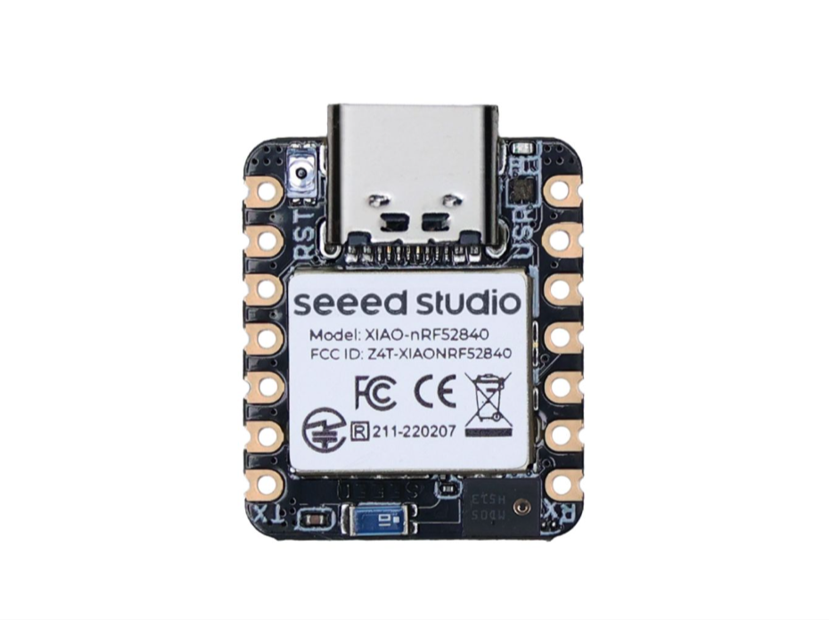
\includegraphics[width=0.5\linewidth]{images/chapter_3/seeed_xiao_nrf52840_sense.png}
        \caption{Seeed XIAO nRF52840 Sense}
        \label{fig:enter-label}
    \end{figure}
    
    Features:
    \begin{itemize}
        \item Powerful wireless capabilities: Bluetooth 5.0 with onboard antenna
        \item Powerful CPU: Nordic nRF52840, ARM® Cortex®-M4 32-bit processor with FPU, 64 MHz
        \item Ultra-Low Power: Standby power consumption is less than 5\(\mu\)A
        \item Battery charging chip: Supports lithium battery charge and discharge management
        \item Onboard 2 MB flash
        \item Onboard PDM microphone (only in Seeed Studio XIAO nRF52840 Sense)
        \item Onboard 6-axis LSM6DS3TR-C IMU (only in Seeed Studio XIAO nRF52840 Sense)
        \item Ultra Small Size: 21 x 17.8mm, Seeed Studio XIAO series classic form-factor for wearable devices
        \item Rich interfaces: 1xUART, 1xI2C, 1xSPI, 1xNFC, 1xSWD, 11xGPIO(PWM), 6xADC in XIAO nRF52840 (Sense); and 2xUART, 1xI2C, 2xSPI, 1xI2S, 1xNFC, 1xSWD, 18xGPIO(PWM), 6xADC in XIAO nRF52840 (Sense) Plus
        \item Single-sided components, surface mounting design
    \end{itemize}
    
    \begin{figure}[!htb]
        \centering
        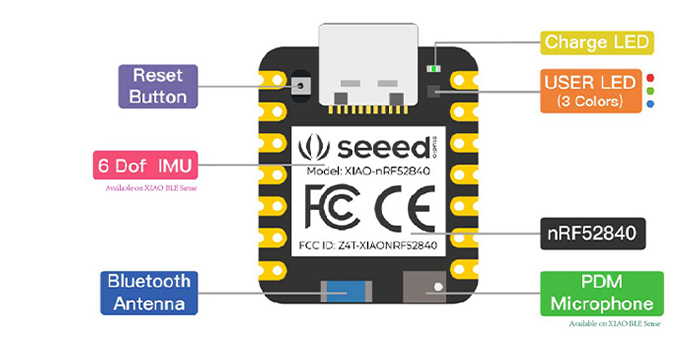
\includegraphics[width=0.5\linewidth]{images/chapter_3/XIAO nRF52840 Sense front indication.png}
        \caption{XIAO nRF52840 Sense front indication}
        \label{fig:enter-label}
    \end{figure}
    \begin{figure}[!htb]
        \centering
        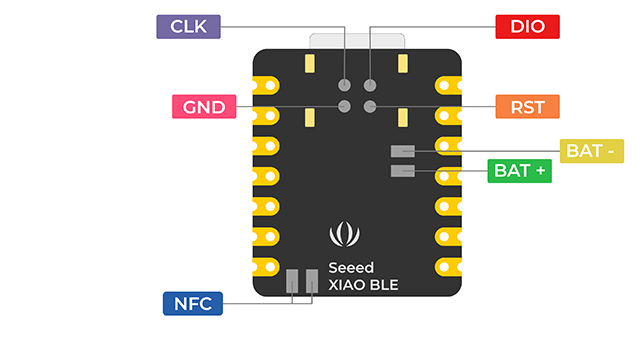
\includegraphics[width=0.5\linewidth]{images/chapter_3/XIAO nRF52840 Sense back indication.png}
        \caption{XIAO nRF52840 Sense back indication}
        \label{fig:enter-label}
    \end{figure}
    \begin{figure}[!htb]
        \centering
        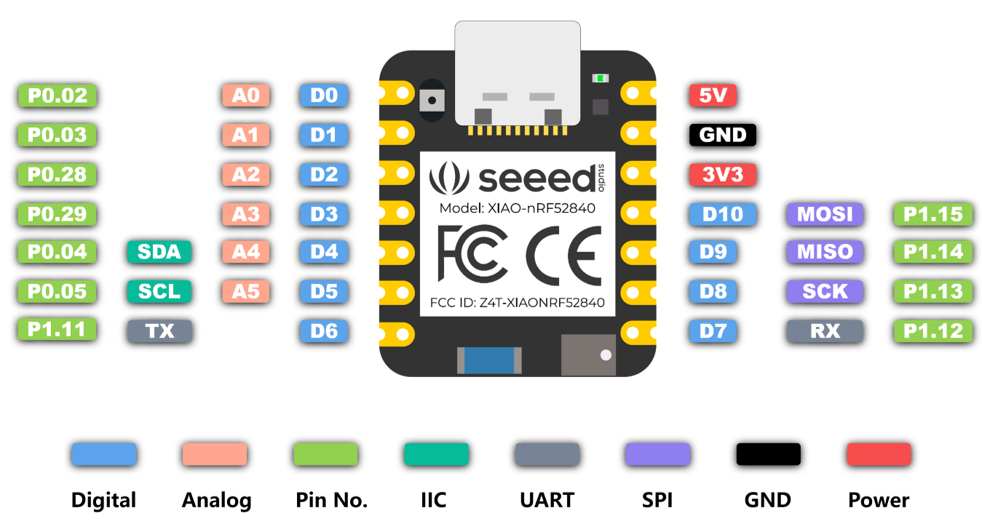
\includegraphics[width=0.6\linewidth]{images/chapter_3/XIAO nRF52840 Sense Pin List.png}
        \caption{XIAO nRF52840 Sense Pin List}
        \label{fig:enter-label}
    \end{figure}

    The built-in IMU sensor details: LSM6DS3:
    \begin{itemize}
        \item Accelerometer Range: ±2g to ±16g.
        \item Gyroscope Range: ±125 dps to ±2000 dps.
        \item Sampling Frequency: Configured at 50 Hz to balance accuracy and power consumption.
    \end{itemize}

    Bluetooth Low Energy (BLE):
    \begin{itemize}
        \item Configured to send motion predictions in real-time to a paired smartphone.
        \item Achieved stable connectivity within a range of 10 meters indoors.
    \end{itemize}

\subsection{Setting up}
    We need to prepare the following:
    \begin{itemize}
        \item 1 x Seeed XIAO nRF52840 Sense
        \item 1 x Battery: 3.3V 80mAh
        \item 1 x Device housing with strap
        \item 1 x Computer
        \item 1 x USB Type-C cable
    \end{itemize}
    Connect the Seeed Studio XIAO nRF52840 (Sense) to your computer via a USB Type-C cable.
    \begin{figure}[!htb]
        \centering
        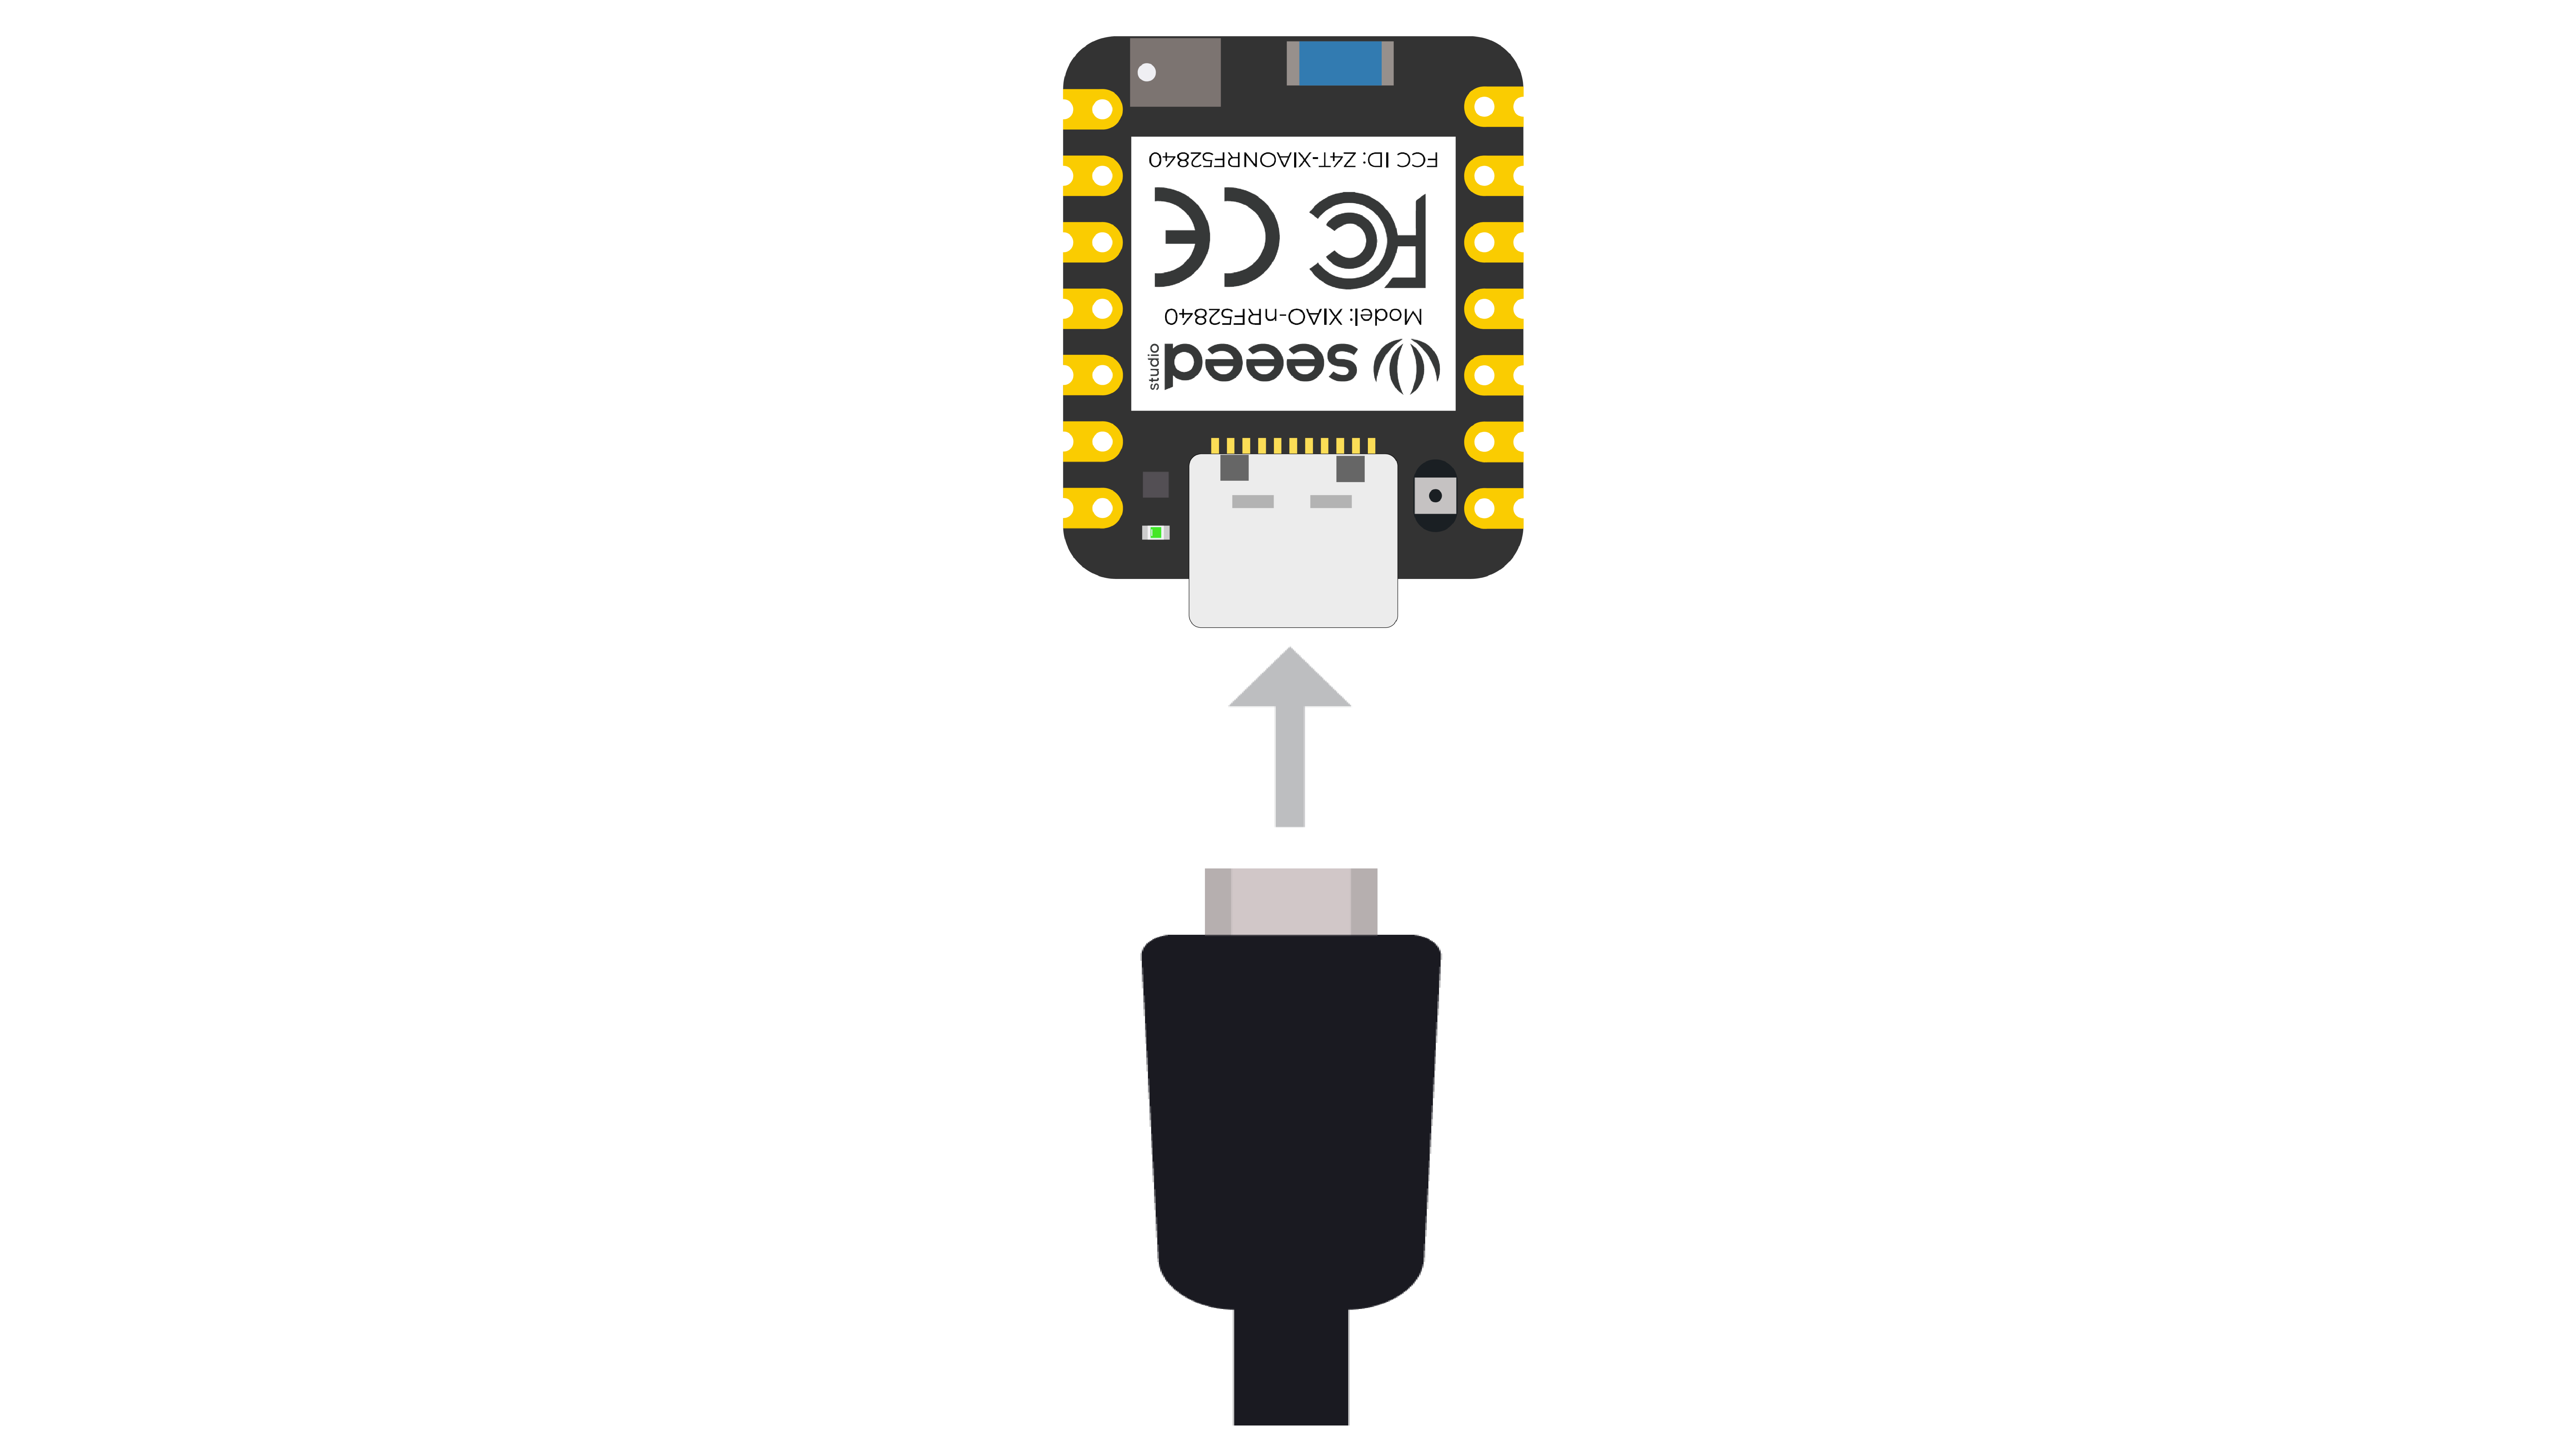
\includegraphics[width=0.5\linewidth]{images/chapter_3/connect_usb_xiao.png}
        \caption{Connect the Seeed Studio XIAO nRF52840 Sense to computer via a USB Type-C cable.}
        \label{fig:enter-label}
    \end{figure}

    \begin{figure}[!htb]
        \centering
        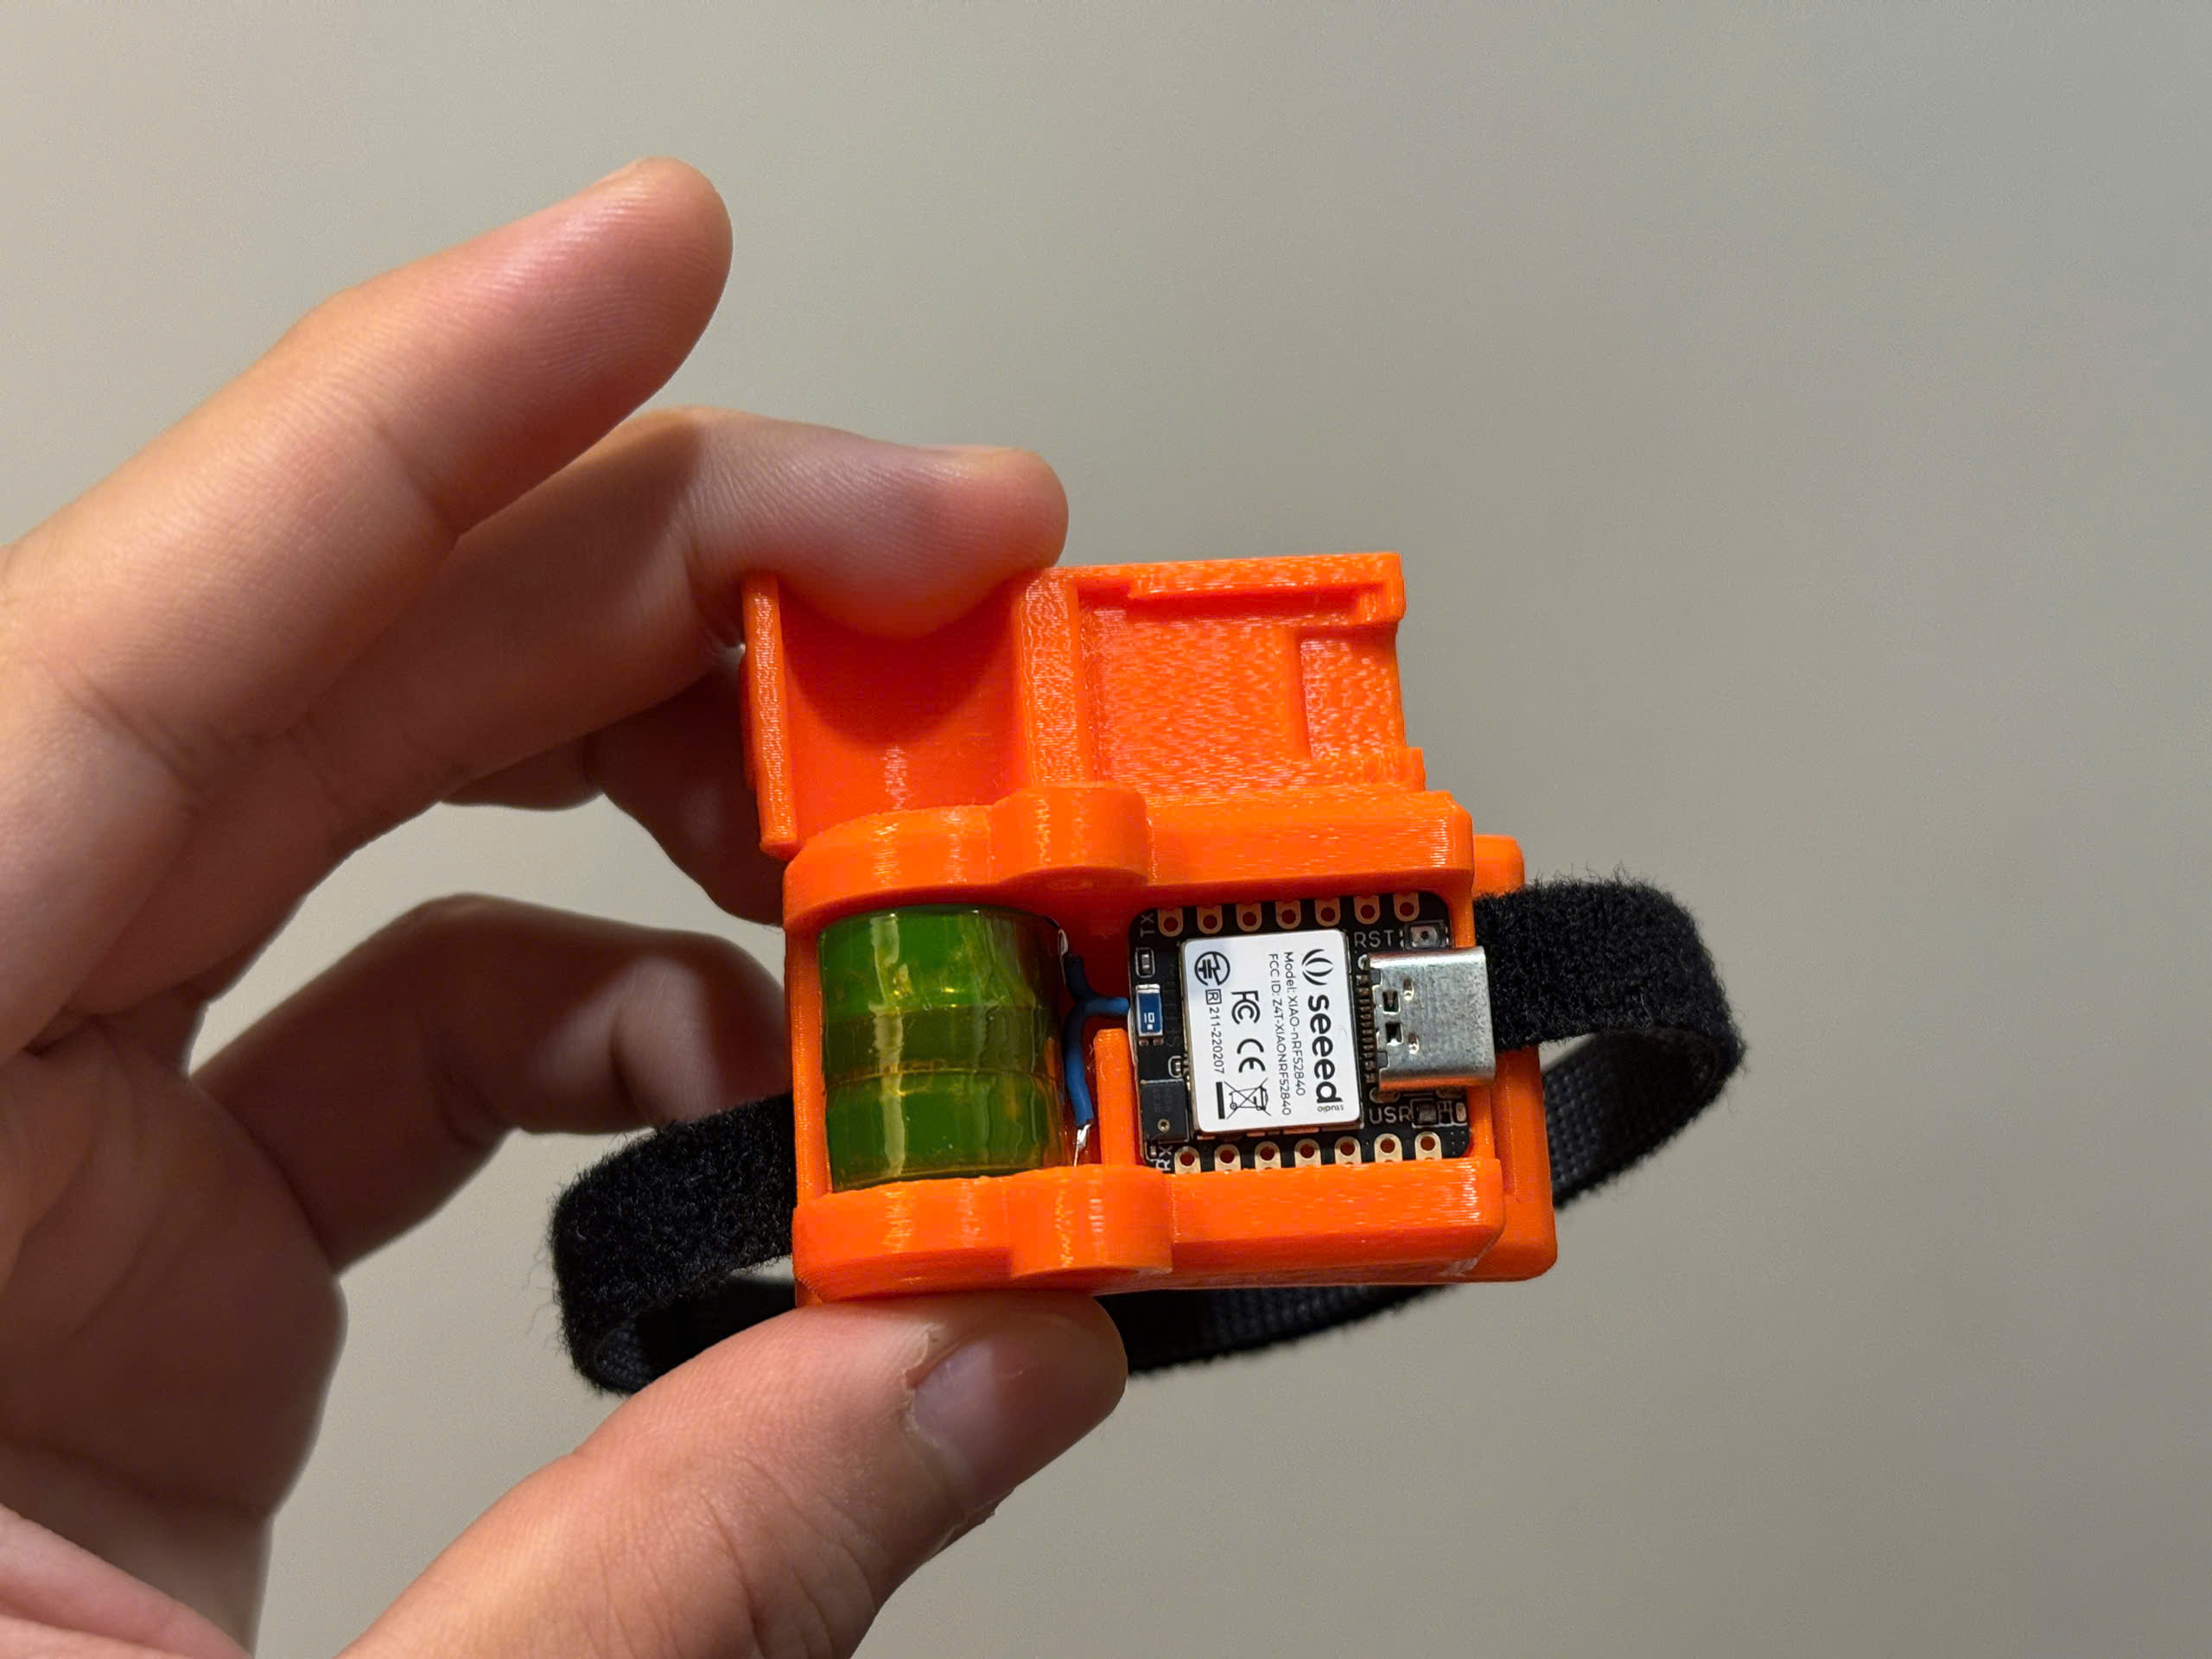
\includegraphics[width=0.5\linewidth]{images/chapter_3/ankle_device_with_battery.png}
        \caption{XIAO nRF52840 with battery}
        \label{fig:enter-label}
    \end{figure}

\section{Software Configuration}

\subsection{Edge Impulse Studio}
    Edge Impulse Studio served as the main platform for the AI workflow:
    
    \begin{enumerate}
        \item Data Acquisition: Collected raw IMU data from the XIAO.
        \item Signal Processing: Extracted relevant motion features using built-in spectral analysis tools.
        \item Model Training: Automated training pipeline with options for real-time accuracy evaluation.
        \item Deployment: Converted trained models to optimized TinyML formats compatible with the XIAO.
    \end{enumerate}

    There is a draw back when directly capturing IMU data using Edge Impulse Studio is that it cannot recognize the gyroscope parameters from the built-in LSM6DS3. Hence, the experiment will use the UART communication to read the serial data from the board.

    

\subsection{Arduino IDE}
Used for firmware programming to enable:

\begin{itemize}
    \item Sensor data streaming via BLE.
    \item Integration with Edge Impulse firmware for model inference.
\end{itemize}

To setup the working environment, the preparation should follow the below steps:

\begin{itemize}
    \item Step 1. Download and Install the latest version of Arduino IDE according to your operating system.
    \item Step 2. Launch the Arduino application
    \item Step 3. Add Seeed Studio XIAO nRF52840 (Sense) board package to your Arduino IDE
        Navigate to File \textgreater Preferences, and fill "Additional Boards Manager URLs" with the url: \url{https://files.seeedstudio.com/arduino/package_seeeduino_boards_index.json}
        
        Navigate to Tools \textgreater Board \textgreater Boards Manager..., type the keyword "seeed nrf52" in the search box, select the latest version of the board you want, and install it. You can install both.
        
        It is recommended to use the \textbf{Seeed nRF52 mbed-enabled Boards} library if you want to use it in embedded Machine Learning Applications or apply "IMU and PDM advanced function".
    \item Step 4. Download and install the supported library from Seeed Studio to work with the built-in IMU easily: \href{https://github.com/Seeed-Studio/Seeed_Arduino_LSM6DS3}{Seeed Arduino LSM6DS3}.
\end{itemize}

\section{Data Acquisition}
\subsection{Data collection}
    \begin{enumerate}
    \item Sensor Placement
    
        Device affixed to the ankle using a strap for stability and consistent positioning.
        \begin{figure}[!htb]
            \centering
            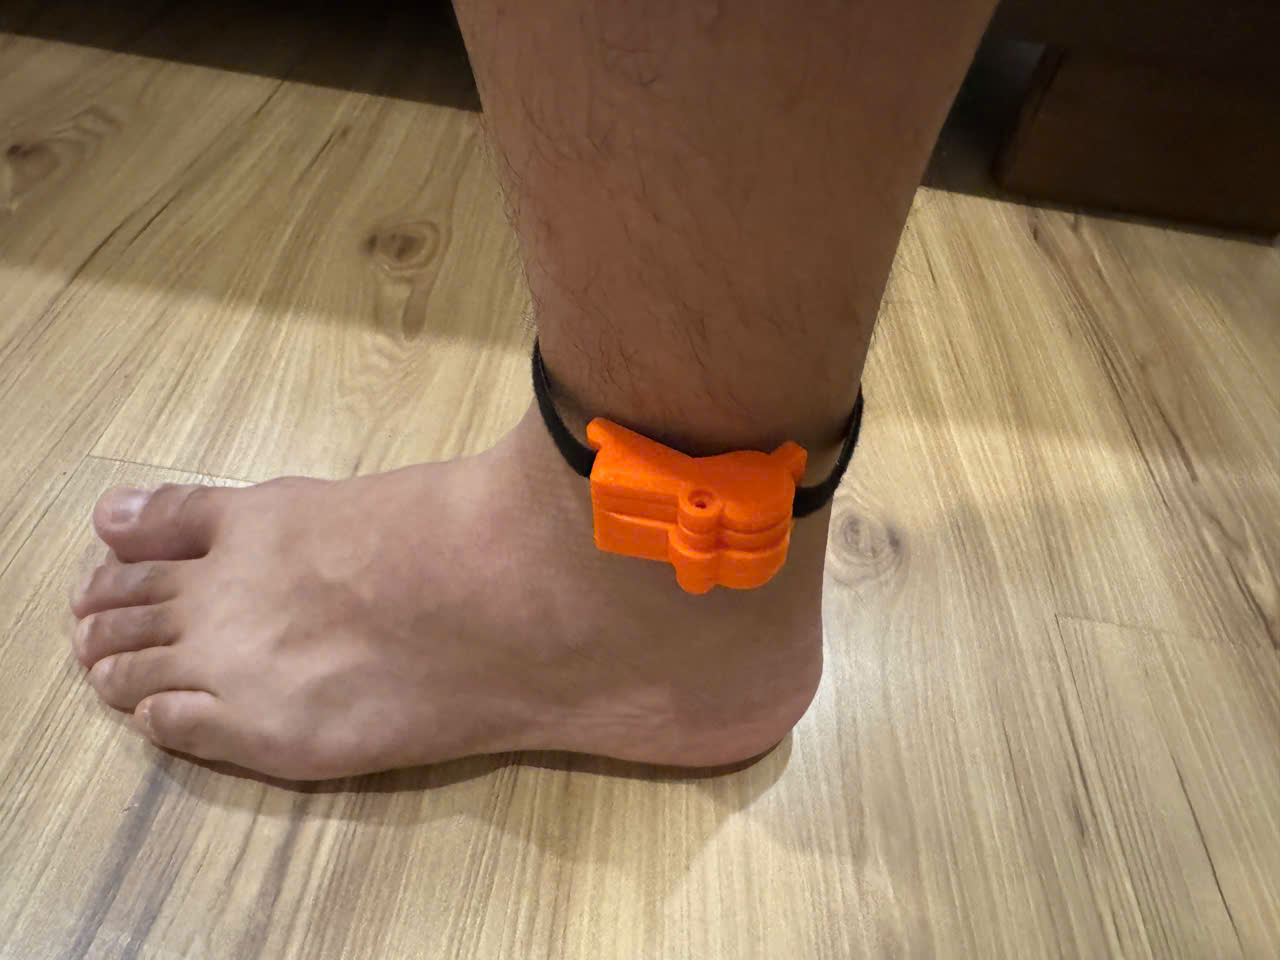
\includegraphics[width=0.5\linewidth]{images/chapter_3/device_affixed_to_ankle.png}
            \caption{Device affixed to ankle}
            \label{fig:enter-label}
        \end{figure}

    \item Recording
    
        Each activity was recorded for around 30 seconds using Arduino sketch to capture serial data. The sampling frequency using is 100Hz. One notice that the IMU address of the device is \textbf{0x6A}

        \begin{lstlisting}[language=C++]
        // XIAO BLE Sense LSM6DS3 Accelerometer Raw Data

        #include "LSM6DS3.h"
        
        // Create a instance of class LSM6DS3
        LSM6DS3 myIMU(I2C_MODE, 0x6A);  // I2C device address 0x6A
        
        #define CONVERT_G_TO_MS2 9.80665f
        #define FREQUENCY_HZ 100
        #define INTERVAL_MS (1000 / (FREQUENCY_HZ + 1))
        
        static unsigned long last_interval_ms = 0;
        
        void setup() {
          Serial.begin(115200);
          while (!Serial)
            ;
        
          if (myIMU.begin() != 0) {
            Serial.println("Device error");
          } else {
            Serial.println("aX,aY,aZ,gX,gY,gZ");
          }
        }
        
        void loop() {
          if (millis() > last_interval_ms + INTERVAL_MS) {
            last_interval_ms = millis();
            Serial.print(myIMU.readFloatAccelX() * CONVERT_G_TO_MS2, 4);
            Serial.print(',');
            Serial.print(myIMU.readFloatAccelY() * CONVERT_G_TO_MS2, 4);
            Serial.print(',');
            Serial.print(myIMU.readFloatAccelZ() * CONVERT_G_TO_MS2, 4);
            Serial.print(',');
            Serial.print(myIMU.readFloatGyroX() * CONVERT_G_TO_MS2, 4);
            Serial.print(',');
            Serial.print(myIMU.readFloatGyroY() * CONVERT_G_TO_MS2, 4);
            Serial.print(',');
            Serial.println(myIMU.readFloatGyroZ() * CONVERT_G_TO_MS2, 4);
          }
        }
        \end{lstlisting}
    \item Labeling
    
        Manual labeling during data acquisition to map samples to their respective activities.
    \end{enumerate}

    \begin{figure}[!htb]
        \centering
        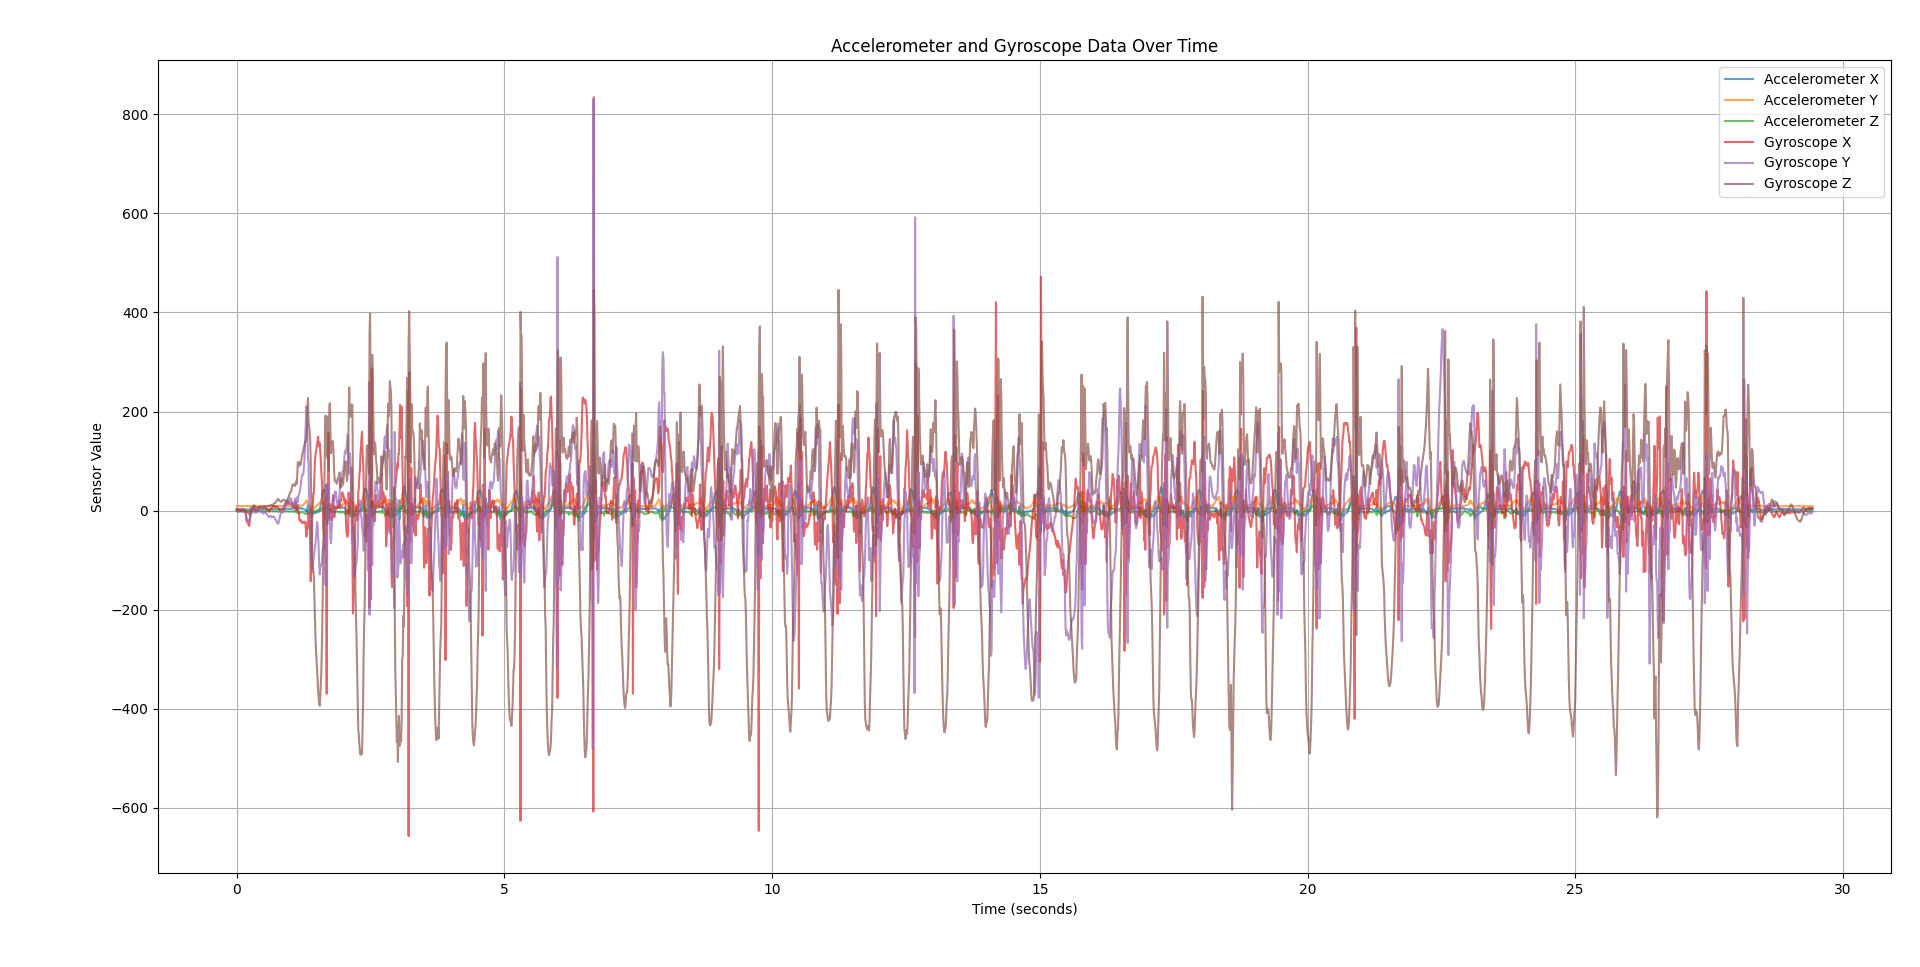
\includegraphics[width=1\linewidth]{images/chapter_3/running_100hz_raw.png}
        \caption{Raw data (100Hz): Running}
        \label{fig:enter-label}
    \end{figure}

    \pagebreak
    
    \begin{figure}[!htb]
        \centering
        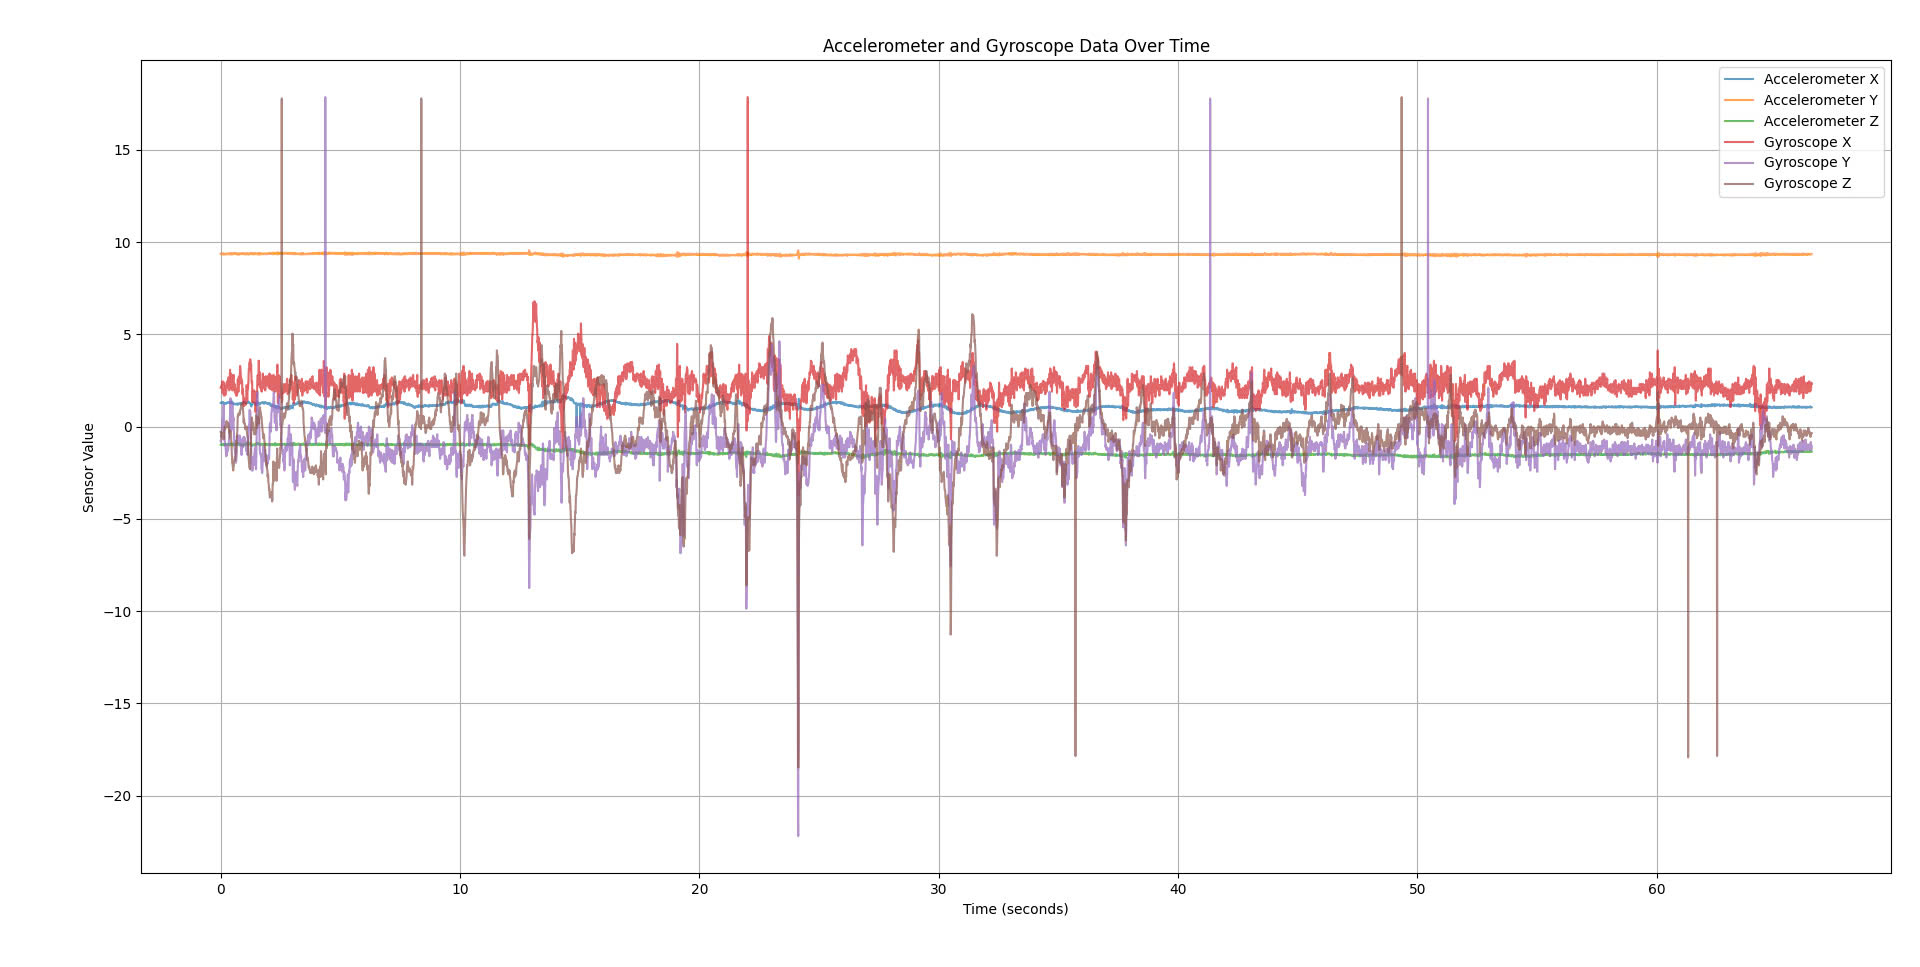
\includegraphics[width=1\linewidth]{images/chapter_3/standing_100hz_raw.png}
        \caption{Raw data (100Hz): Standing}
        \label{fig:enter-label}
    \end{figure}
    \begin{figure}[!htb]
        \centering
        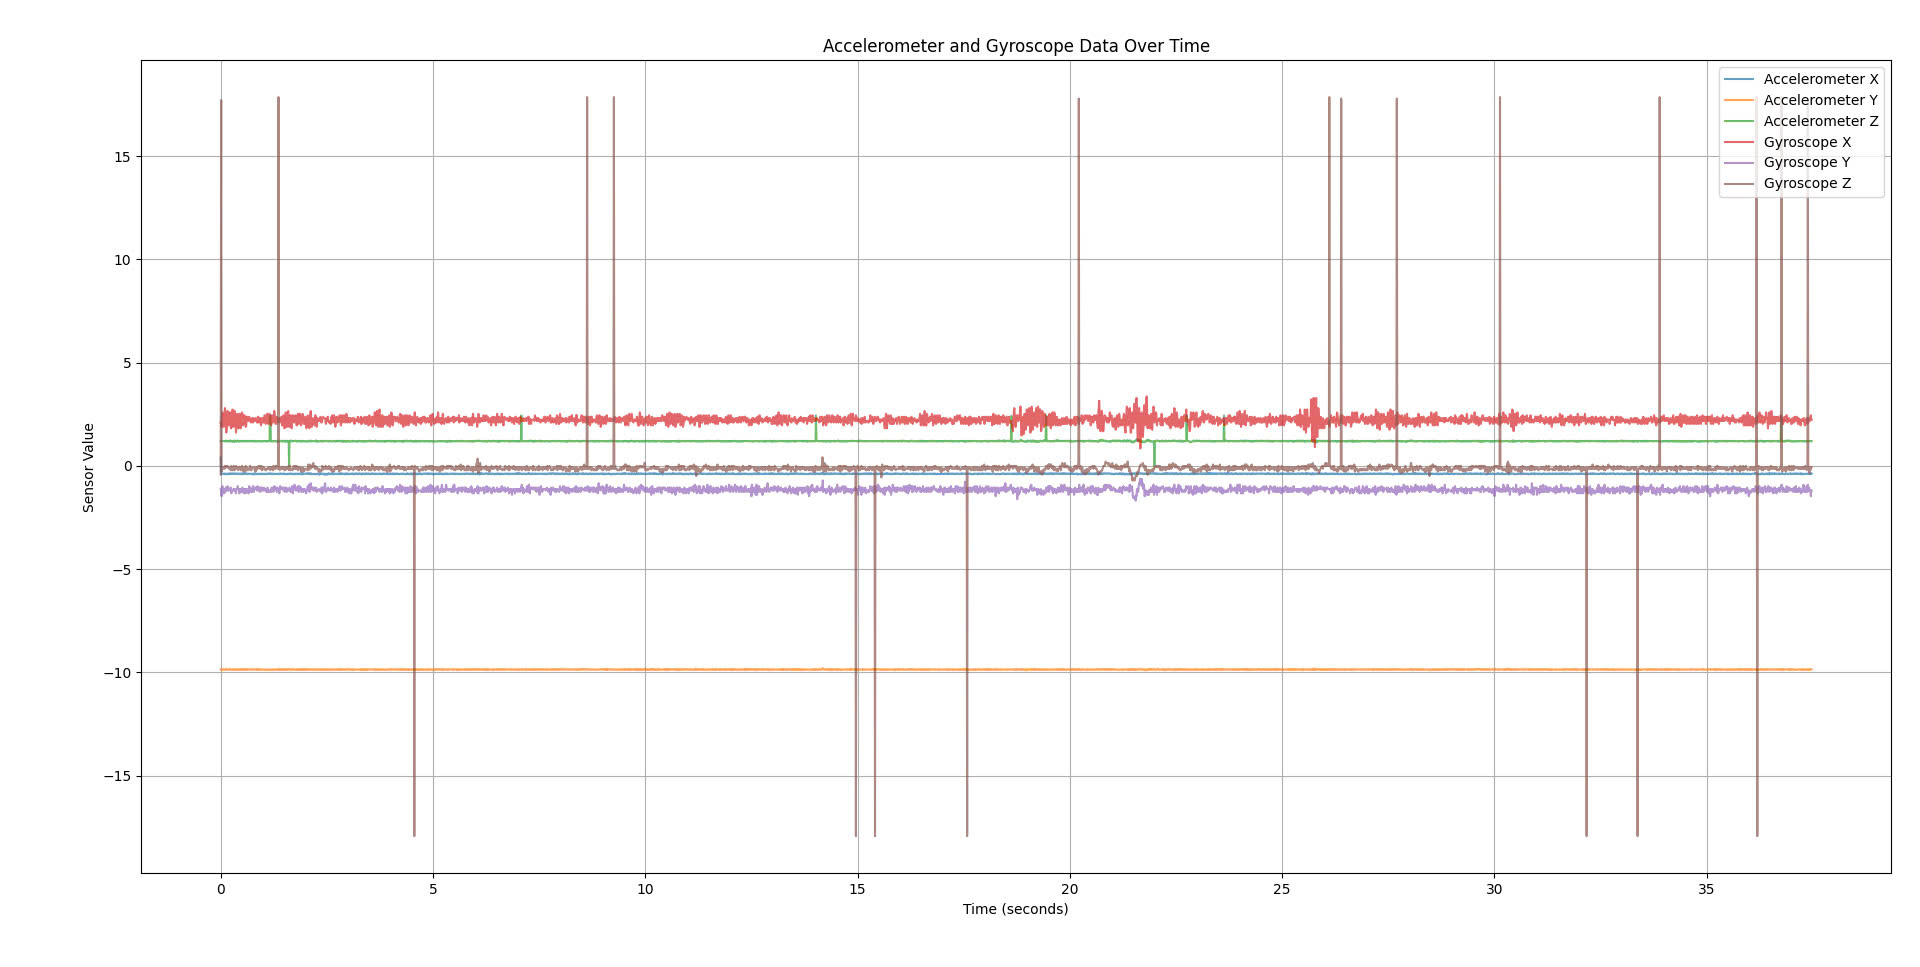
\includegraphics[width=1\linewidth]{images/chapter_3/notwearing_100hz_raw.png}
        \caption{Raw data (100Hz): Not wearing}
        \label{fig:enter-label}
    \end{figure}
    
    \pagebreak
    
    \begin{figure}[!htb]
        \centering
        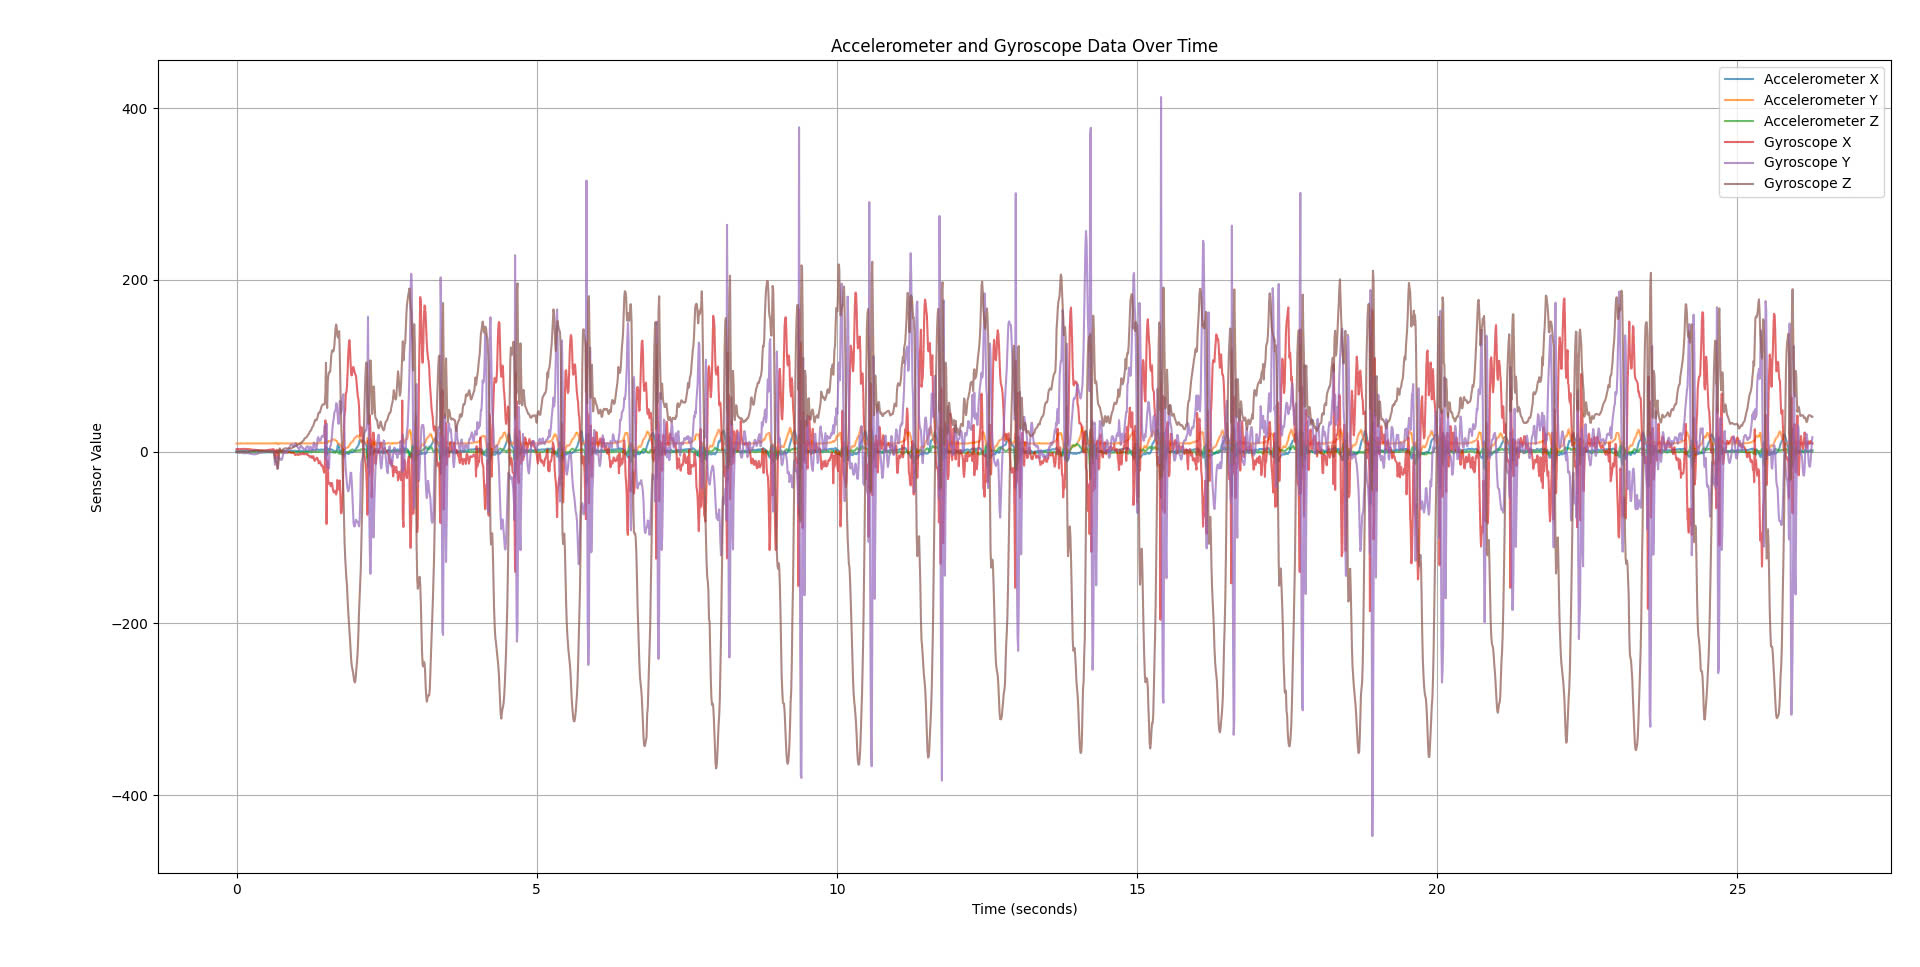
\includegraphics[width=1\linewidth]{images/chapter_3/walking_100hz_raw.png}
        \caption{Raw data (100Hz): Walking}
        \label{fig:enter-label}
    \end{figure}
    \begin{figure}[!htb]
        \centering
        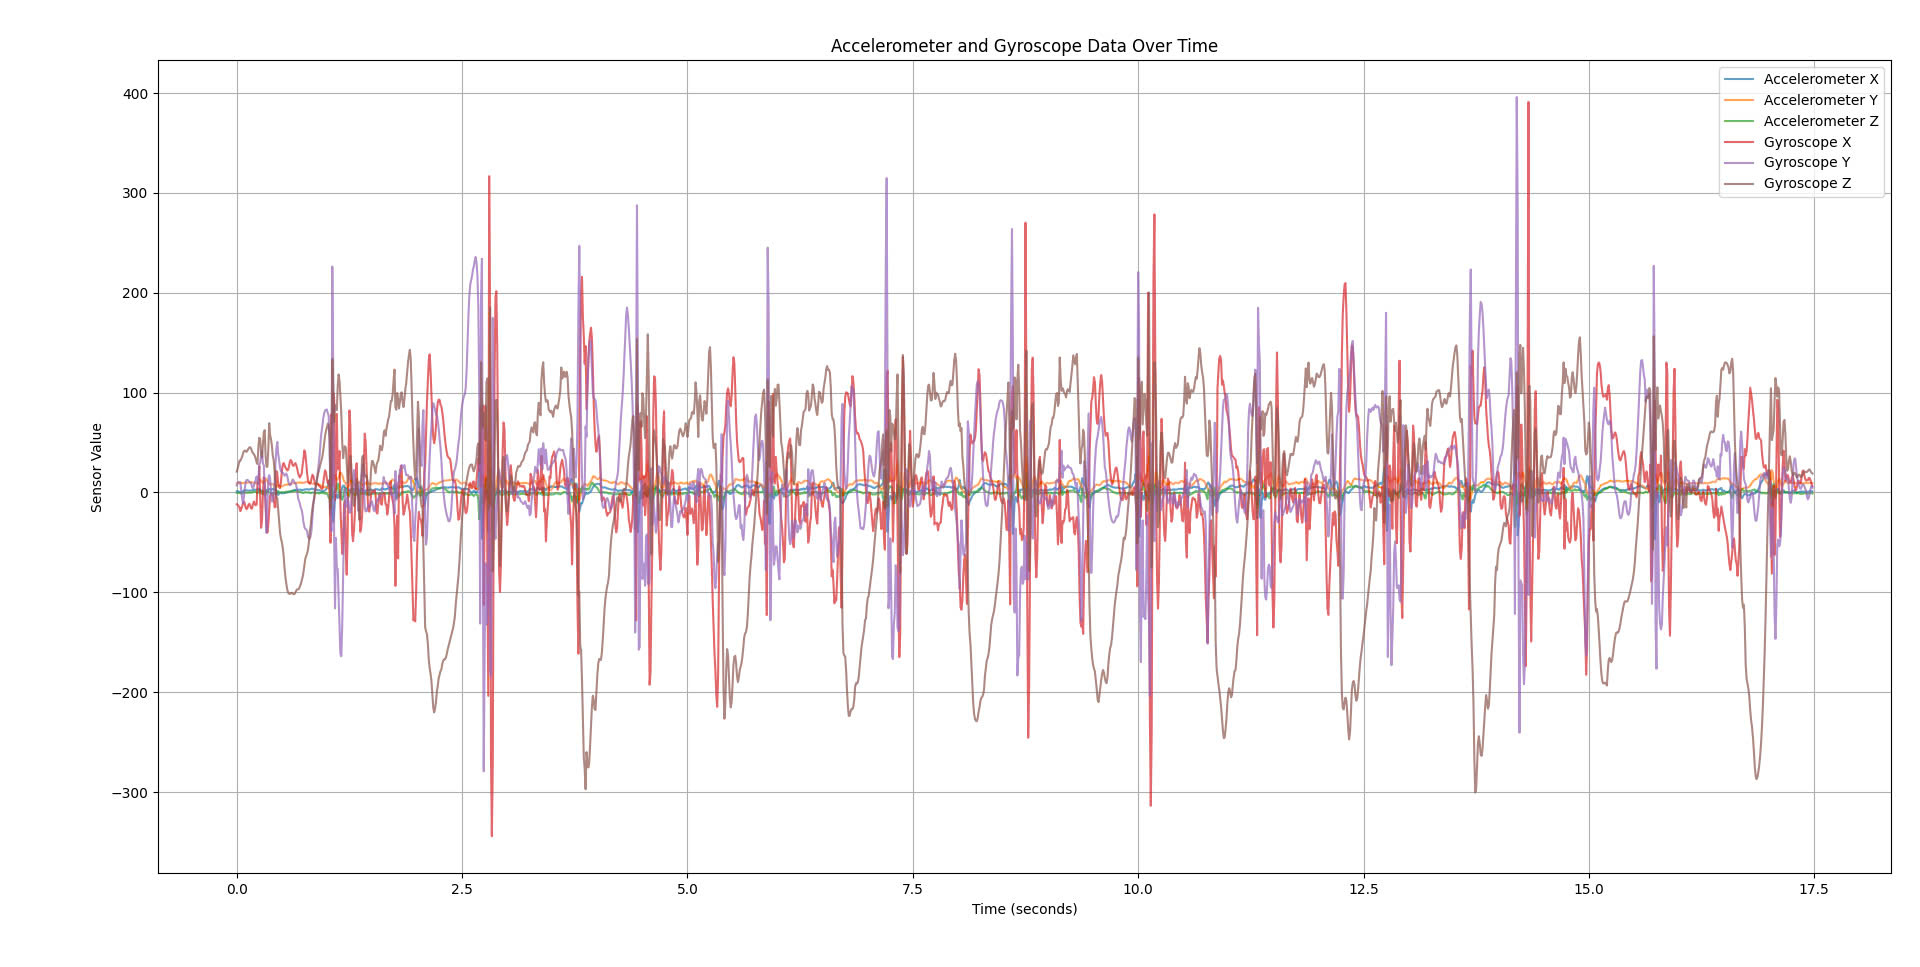
\includegraphics[width=1\linewidth]{images/chapter_3/walkingdownstairs_100hz_raw.png}
        \caption{Raw data (100Hz): Walking downstairs}
        \label{fig:enter-label}
    \end{figure}

    \pagebreak

    \begin{figure}[!htb]
        \centering
        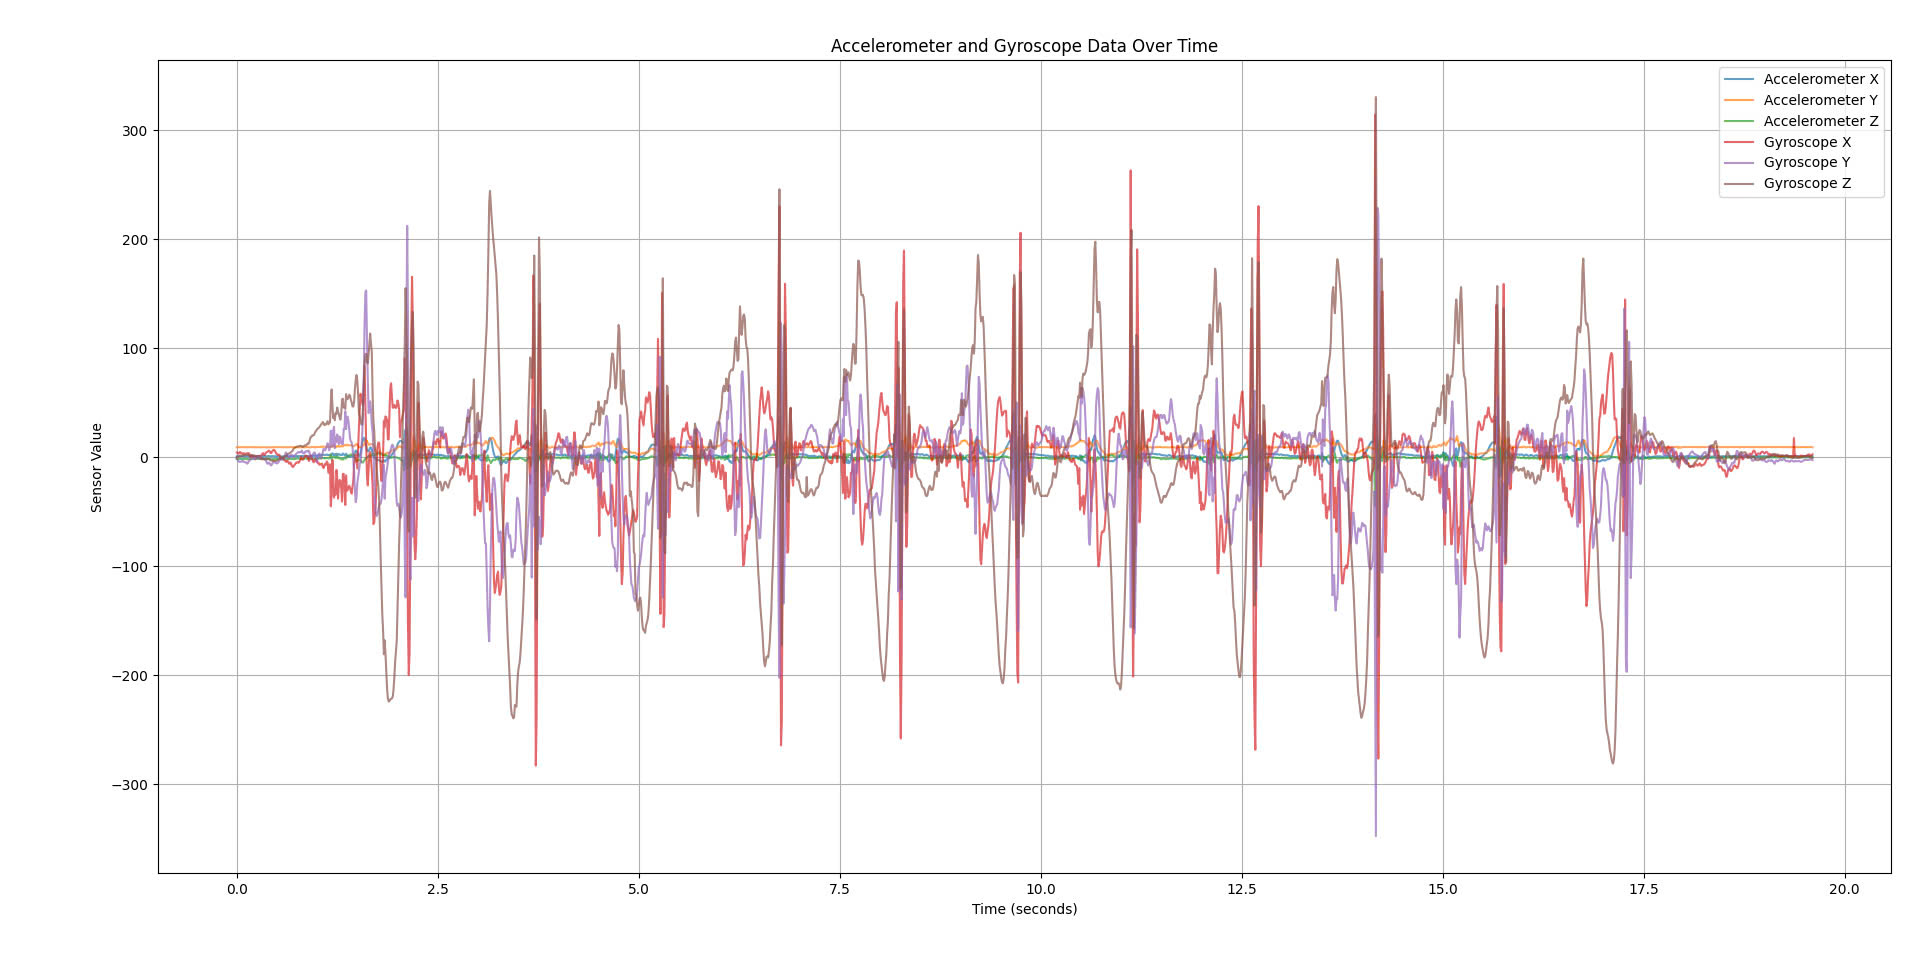
\includegraphics[width=1\linewidth]{images/chapter_3/walkingupstairs_100hz_raw.png}
        \caption{Raw data (100Hz): Walking upstairs}
        \label{fig:enter-label}
    \end{figure}

\subsection{Data preprocessing}
    As the raw data are inconsistent and having many outliers that could lead to the ineffective training results. Therefore, we need to preprocess the data by cleaning and smoothening. To achieve that, Python is a great tool for such job.

    \begin{lstlisting}[language=Python][!htb]
    import pandas as pd
    import numpy as np
    import matplotlib.pyplot as plt
    from scipy.signal import butter, filtfilt
    
    # Load the dataset
    filename = 'walking_upstairs'
    file_path = f'{filename}.csv'  # Replace with the correct file path
    data = pd.read_csv(file_path)
    
    # Specify the IMU columns
    imu_columns = ['aX', 'aY', 'aZ', 'gX', 'gY', 'gZ']
    
    # Function to visualize raw data
    def visualize_data(data, title="IMU Data"):
        plt.figure(figsize=(16, 8))
        for i, col in enumerate(data.columns):
            plt.subplot(2, 3, i + 1)
            plt.plot(data[col], label=col, linewidth=0.8)
            plt.title(f"{col} - {title}")
            plt.xlabel("Samples")
            plt.ylabel("Value")
            plt.legend()
            plt.grid()
        plt.tight_layout()
        plt.show()
    
    # Visualize raw data
    visualize_data(data[imu_columns], title="Raw Data")
    
    # Detect and remove outliers using Z-Score
    def remove_outliers(data, threshold=3):
        z_scores = np.abs((data - data.mean()) / data.std())
        return data[(z_scores < threshold).all(axis=1)]
    
    # Apply outlier removal
    data_cleaned = remove_outliers(data[imu_columns])
    
    # Function to apply a low-pass filter
    def low_pass_filter(data, cutoff=5, fs=50, order=2):
        nyquist = 0.5 * fs
        normal_cutoff = cutoff / nyquist
        b, a = butter(order, normal_cutoff, btype='low', analog=False)
        return pd.DataFrame(filtfilt(b, a, data, axis=0), columns=data.columns)
    
    # Apply low-pass filter
    data_smoothed = low_pass_filter(data_cleaned, cutoff=5, fs=50)
    
    # Visualize cleaned and smoothed data
    visualize_data(data_cleaned, title="Cleaned Data")
    visualize_data(data_smoothed, title="Smoothed Data")
    
    # Save cleaned and smoothed data
    output_cleaned_path = f'{filename}_cleaned.csv'
    output_smoothed_path = f'{filename}_smoothed.csv'
    data_cleaned.to_csv(output_cleaned_path, index=False)
    data_smoothed.to_csv(output_smoothed_path, index=False)
    
    print(f"Cleaned data saved to {output_cleaned_path}")
    print(f"Smoothed data saved to {output_smoothed_path}")
    \end{lstlisting}

    After running the preprocessing job on the raw data, we can get the much better data samples.

    \begin{figure}[!htb]
        \centering
        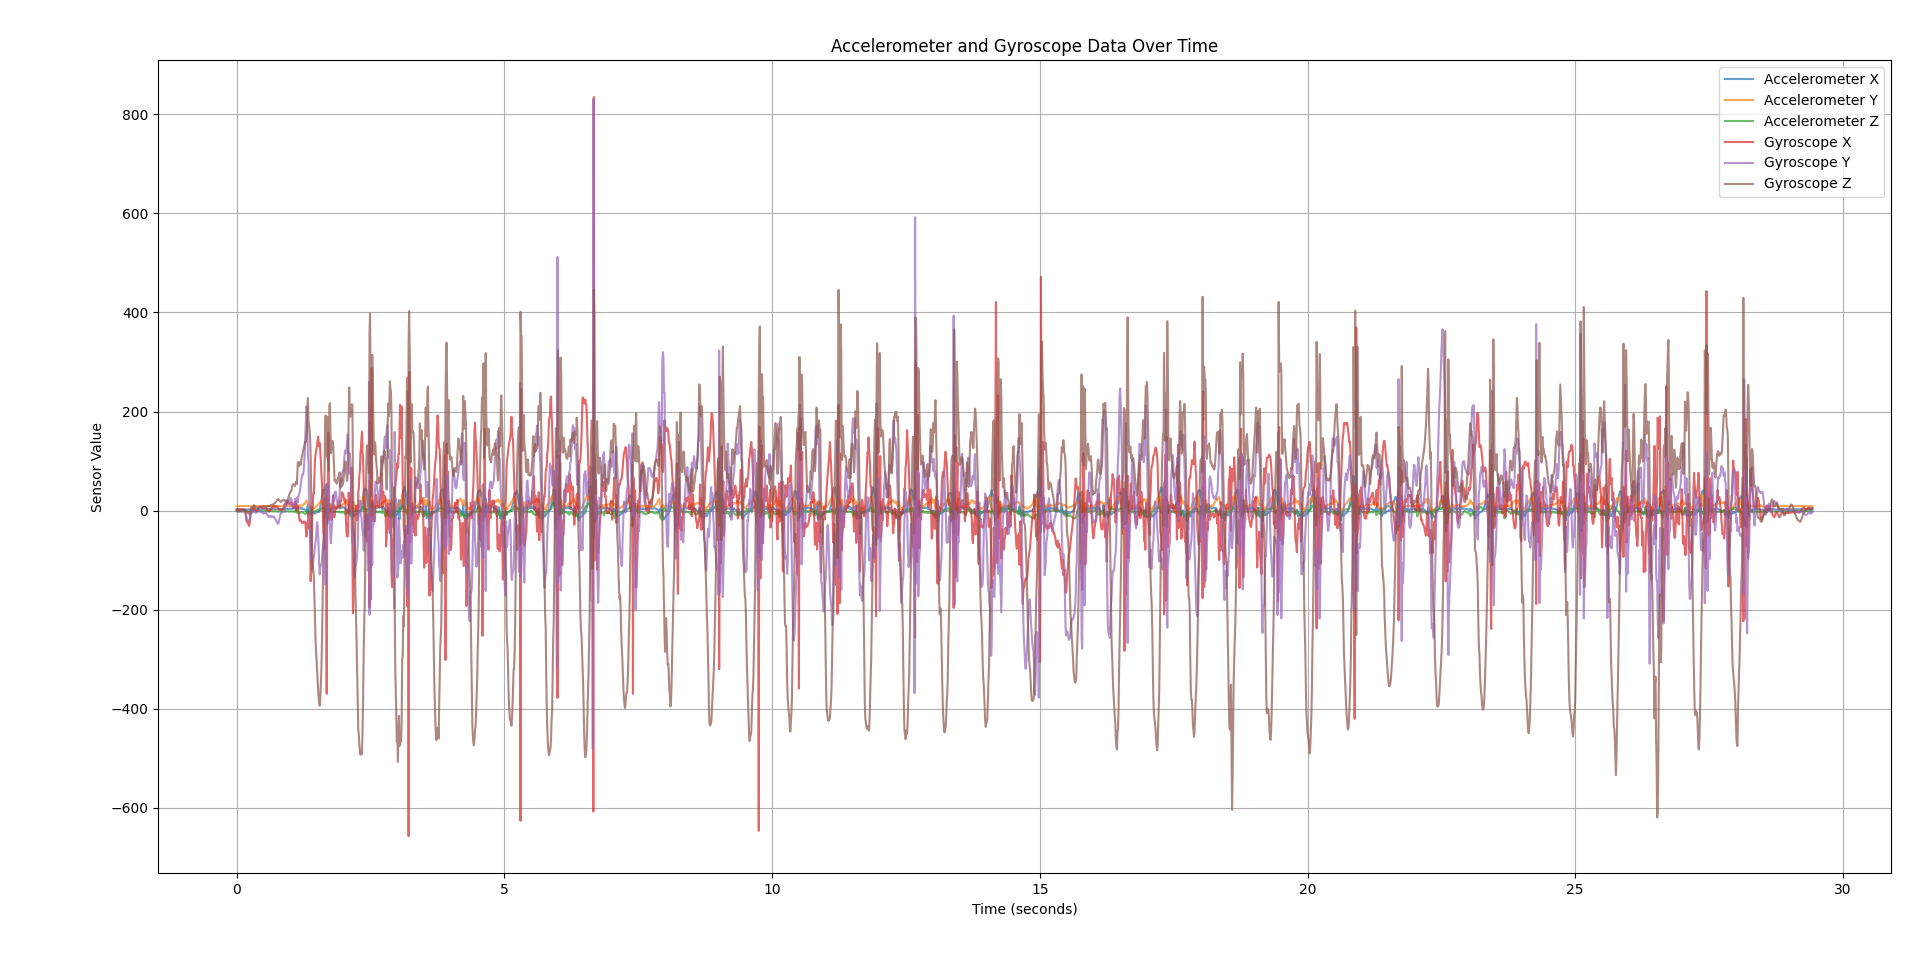
\includegraphics[width=1\linewidth]{images/chapter_3/running_100hz_preprocessed.png}
        \caption{Preprocessed: Running}
        \label{fig:enter-label}
    \end{figure}

    \pagebreak
    
    \begin{figure}[!htb]
        \centering
        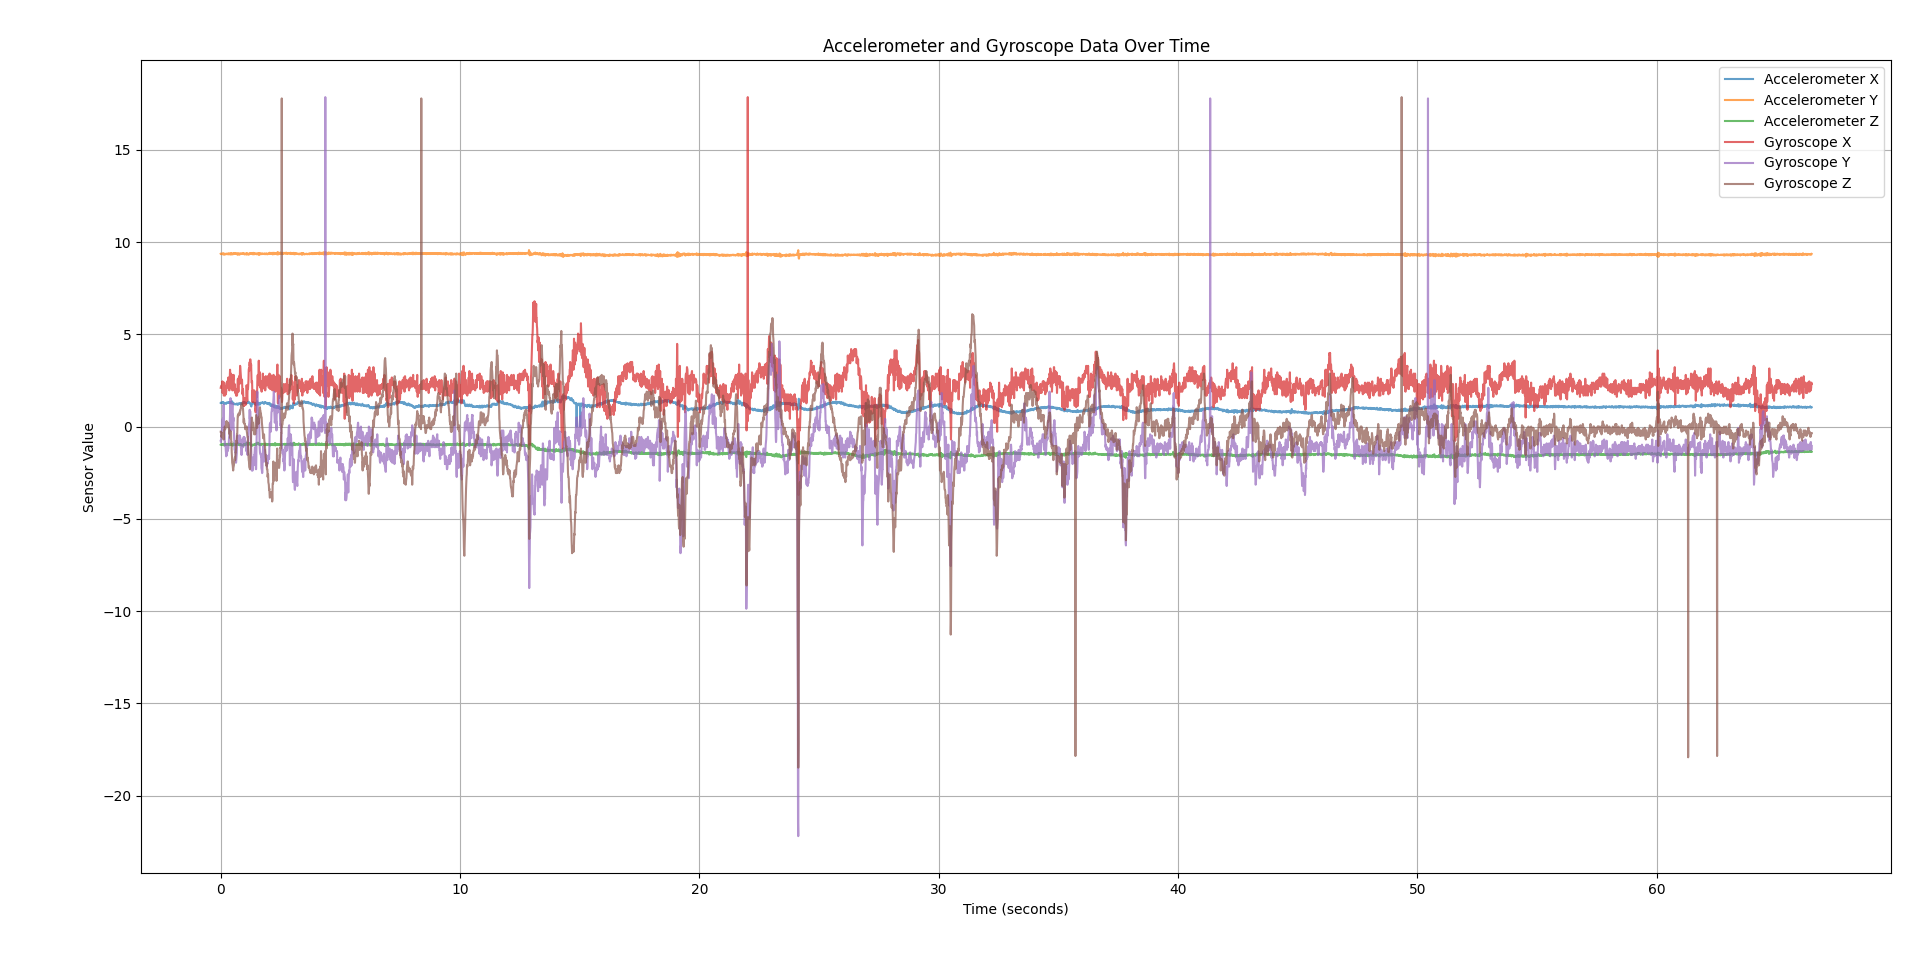
\includegraphics[width=1\linewidth]{images/chapter_3/standing_100hz_preprocessed.png}
        \caption{Preprocessed: Standing}
        \label{fig:enter-label}
    \end{figure}
    \begin{figure}[!htb]
        \centering
        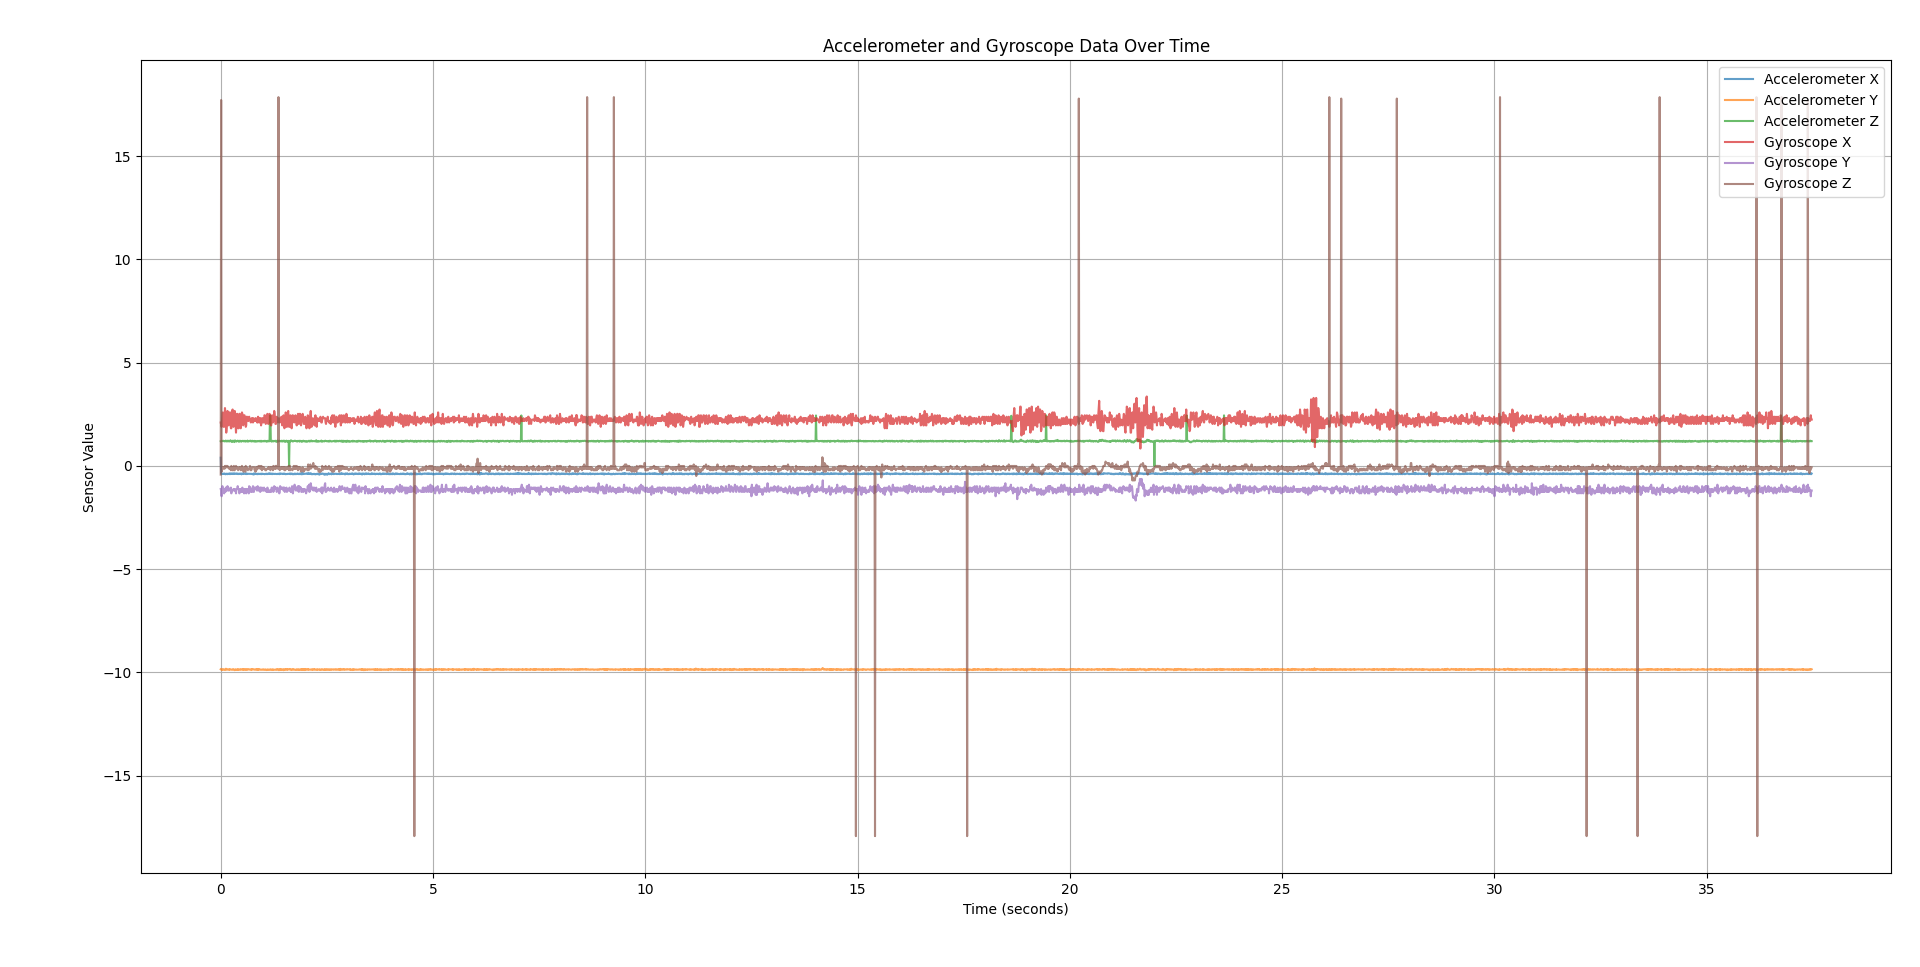
\includegraphics[width=1\linewidth]{images/chapter_3/notwearing_100hz_preprocessed.png}
        \caption{Preprocessed: Not wearing}
        \label{fig:enter-label}
    \end{figure}

    \pagebreak
    
    \begin{figure}[!htb]
        \centering
        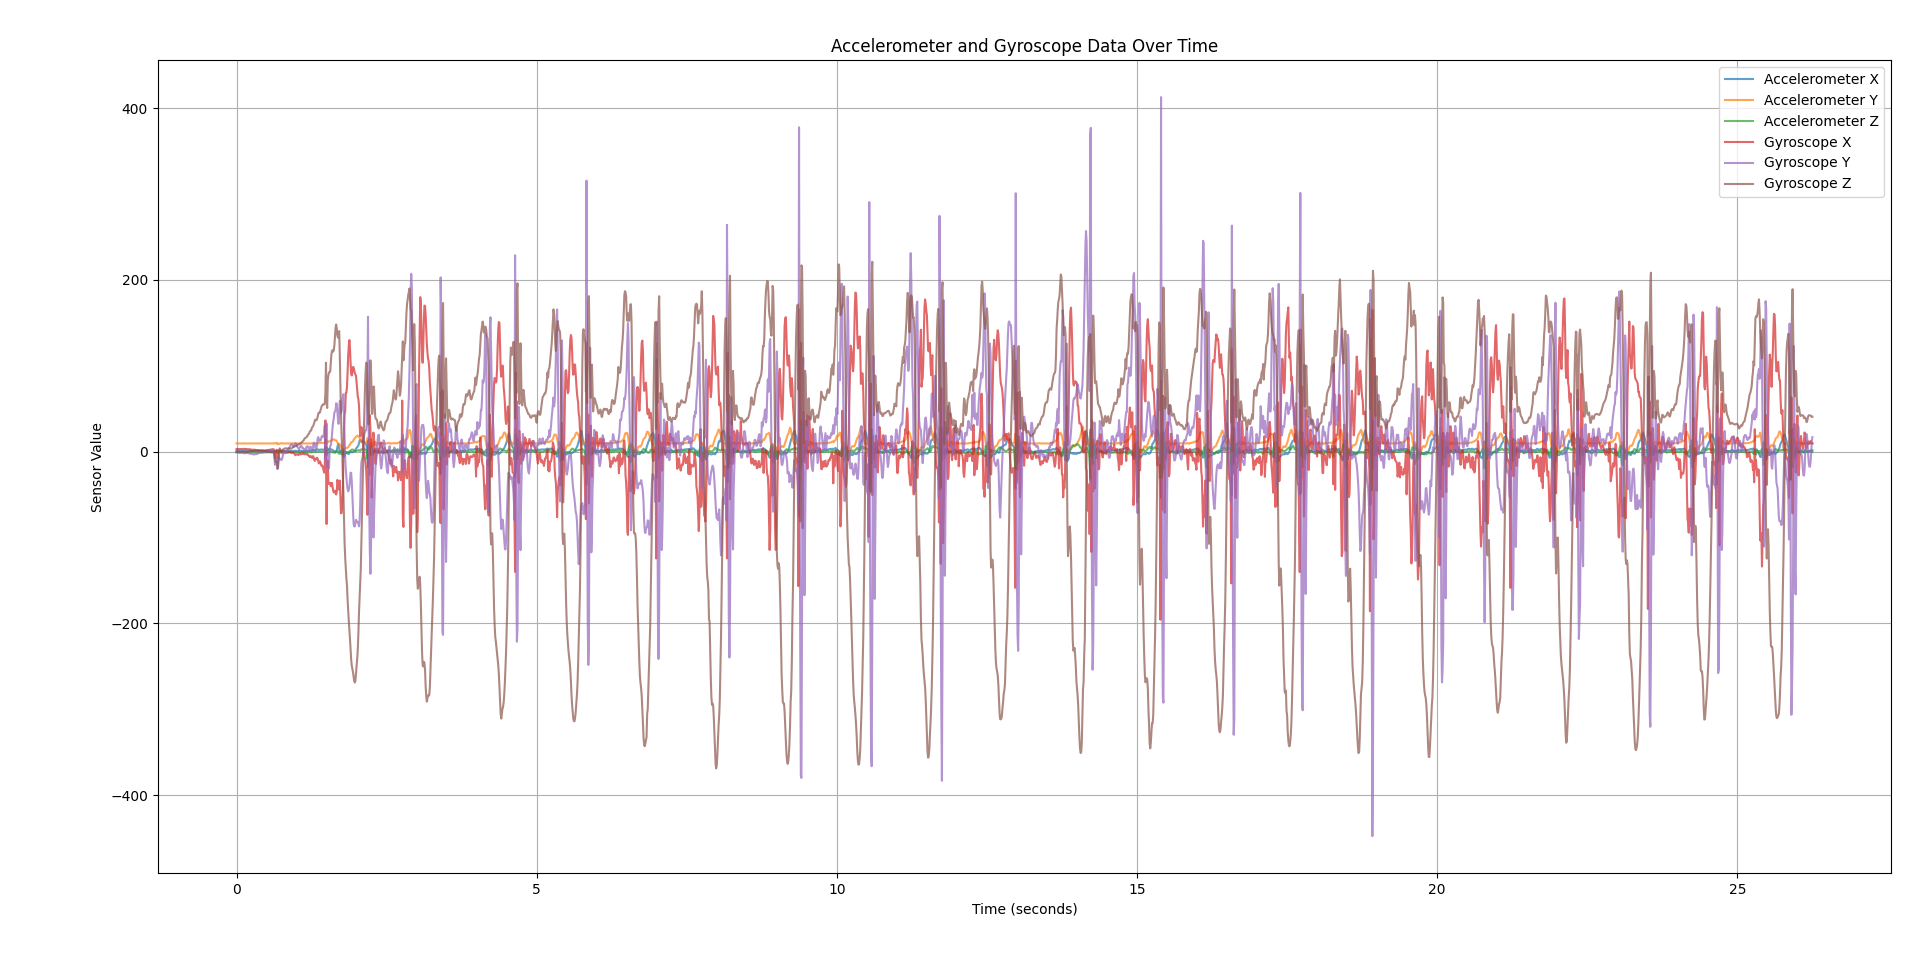
\includegraphics[width=1\linewidth]{images/chapter_3/walking_100hz_preprocessed.png}
        \caption{Preprocessed: Walking}
        \label{fig:enter-label}
    \end{figure}
    \begin{figure}[!htb]
        \centering
        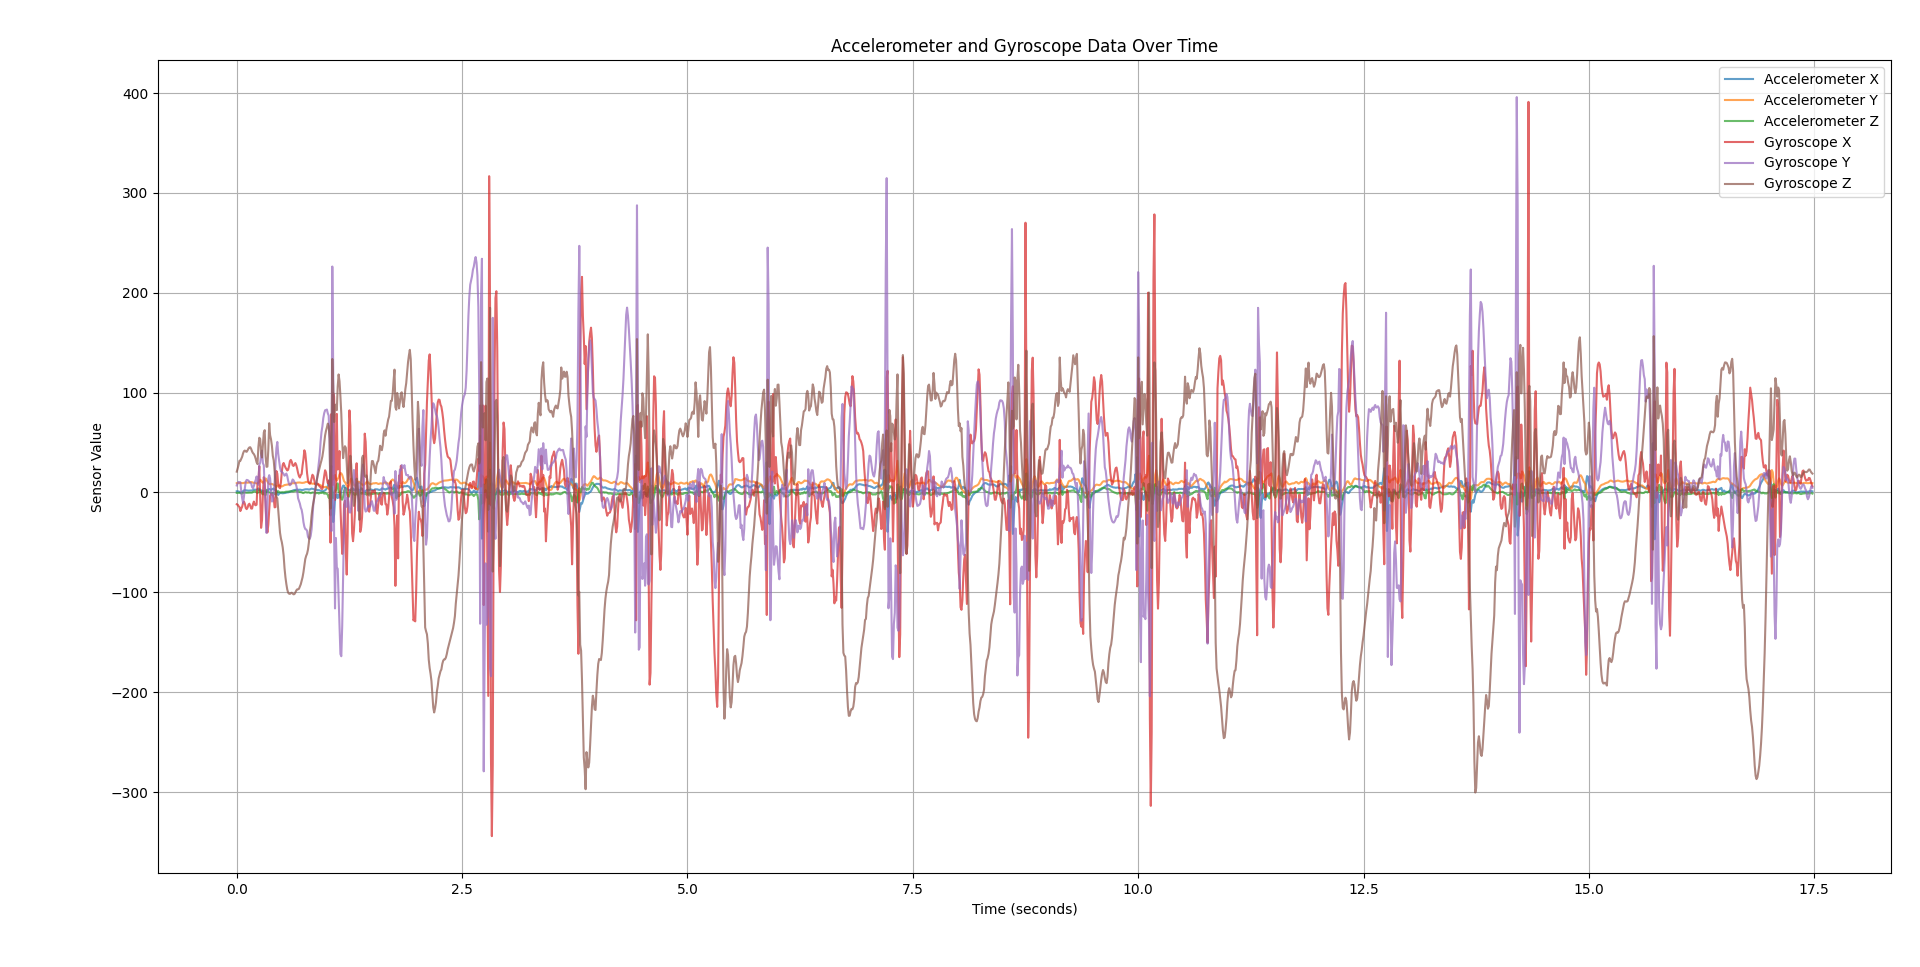
\includegraphics[width=1\linewidth]{images/chapter_3/walkingdownstairs_100hz_preprocessed.png}
        \caption{Preprocessed: Walking downstairs}
        \label{fig:enter-label}
    \end{figure}

    \pagebreak
    
    \begin{figure}[!htb]
        \centering
        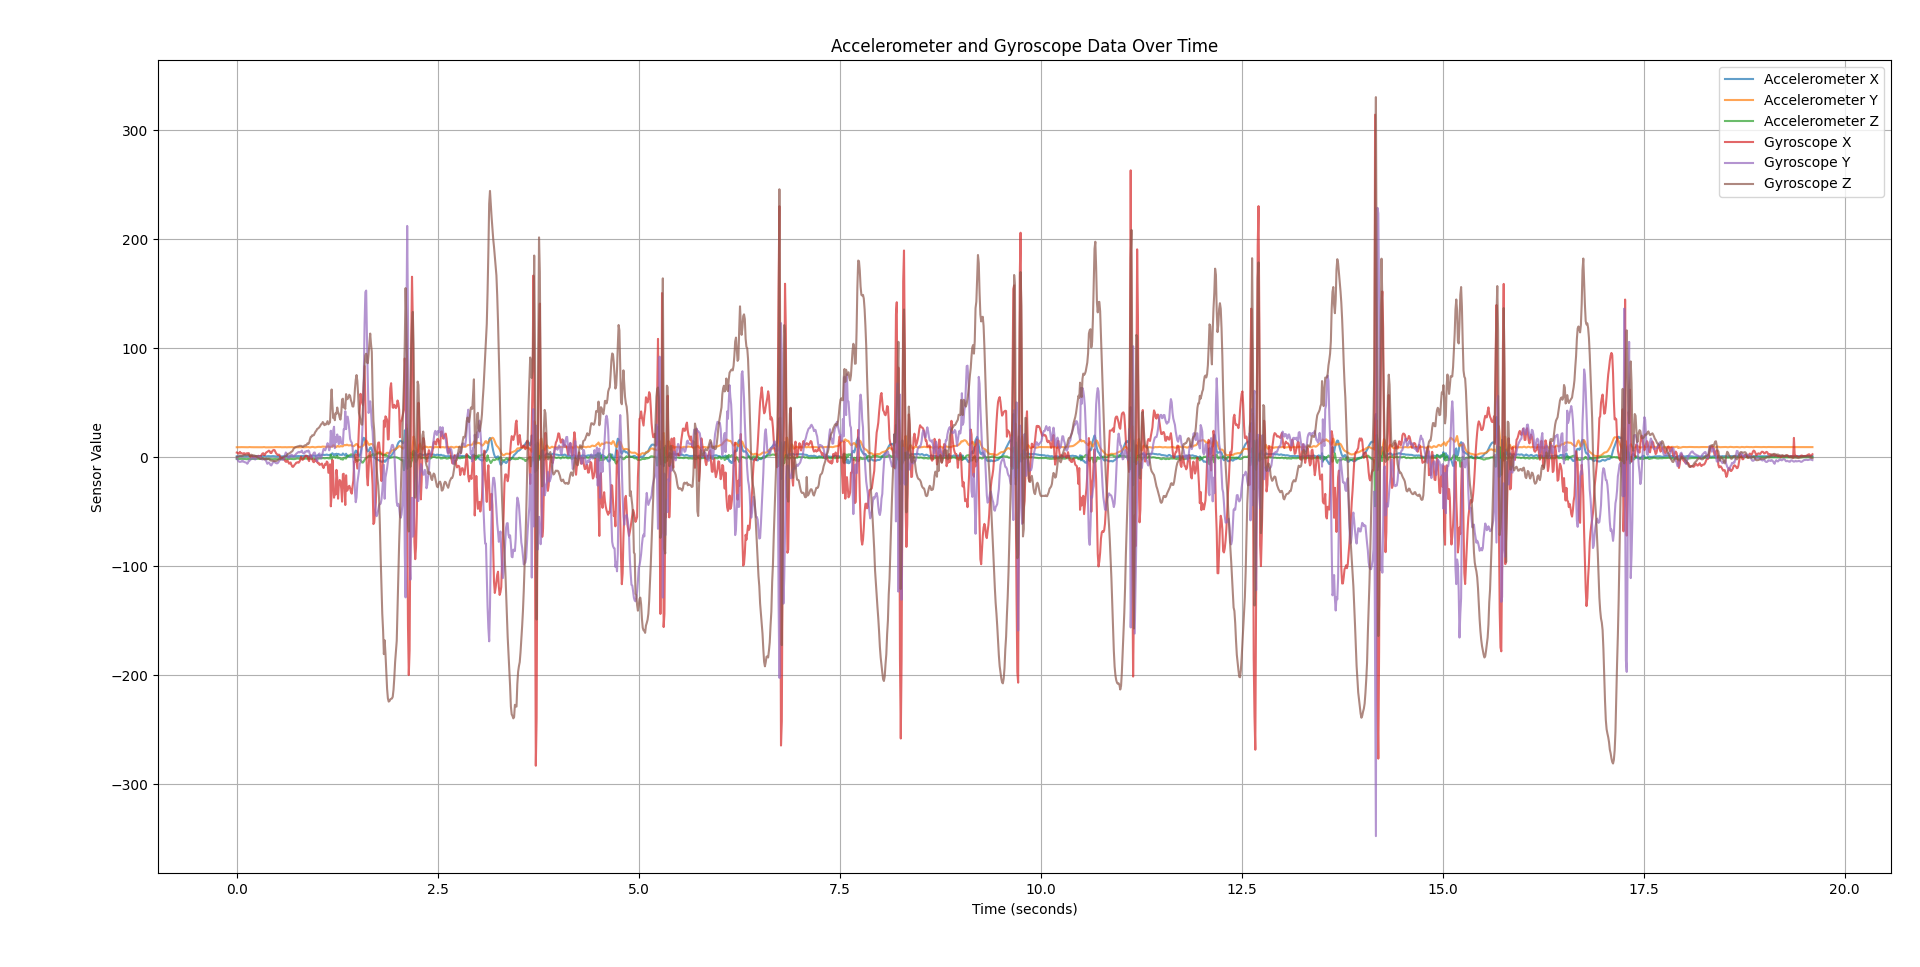
\includegraphics[width=1\linewidth]{images/chapter_3/walkingupstairs_100hz_proprocessed.png}
        \caption{Preprocessed: Walking upstairs}
        \label{fig:enter-label}
    \end{figure}

\section{Model Development}
\subsection{Dataset preparation}
    After having the preprocessed data, the next step is to upload the data samples to Edge Impulse project. 

    \begin{figure}[!htb]
        \centering
        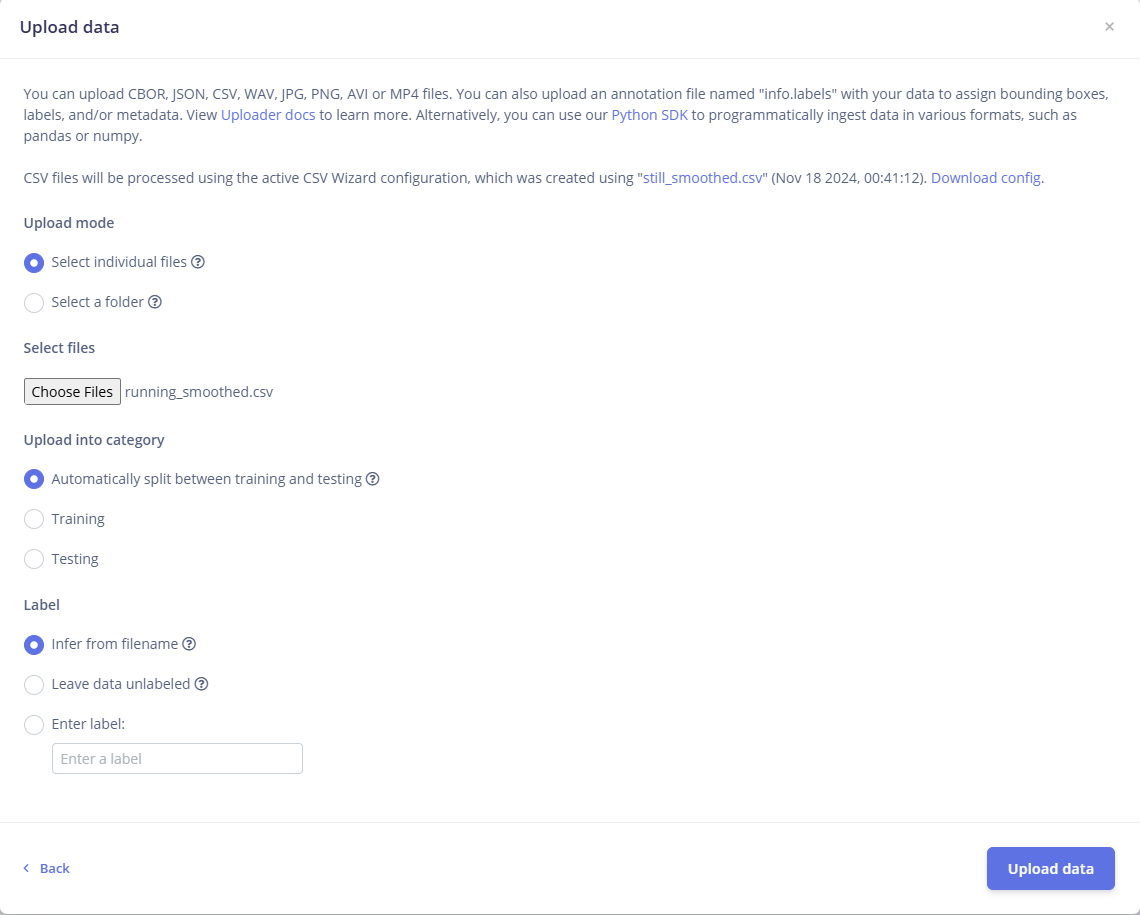
\includegraphics[width=1\linewidth]{images/chapter_3/edgeimpulse_upload_data.png}
        \caption{Edge Impulse Upload data }
        \label{fig:enter-label}
    \end{figure}

    \pagebreak
    After uploading the data, Edge Impulse has a preview panel showing how our data look like. Moreover, it allows us to crop and split the data into multiple small samples with the label from the uploaded data.

    \begin{figure}[!htb]
        \centering
        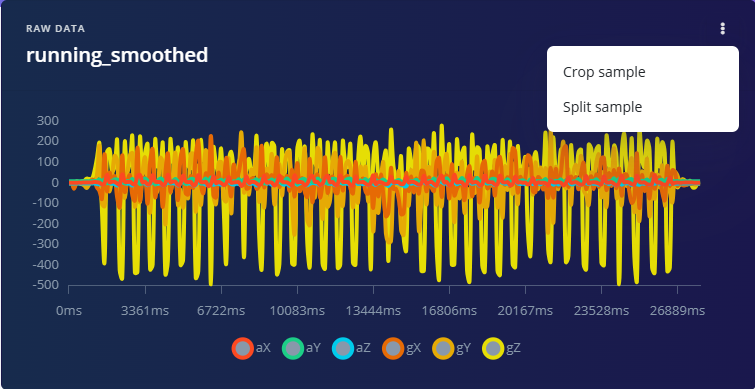
\includegraphics[width=1\linewidth]{images/chapter_3/edgeimpulse_uploaded_data_preview.png}
        \caption{Edge Impulse Uploaded data preview}
        \label{fig:enter-label}
    \end{figure}

    By choosing split sample, Edge Impulse will pop up a window for us to adjust the splitting job. We can adjust the segment length to wider or narrower, or add more segments. After finish, the tool will break our data file into the number of segments that we specify in the split tool.

    \begin{figure}[!htb]
        \centering
        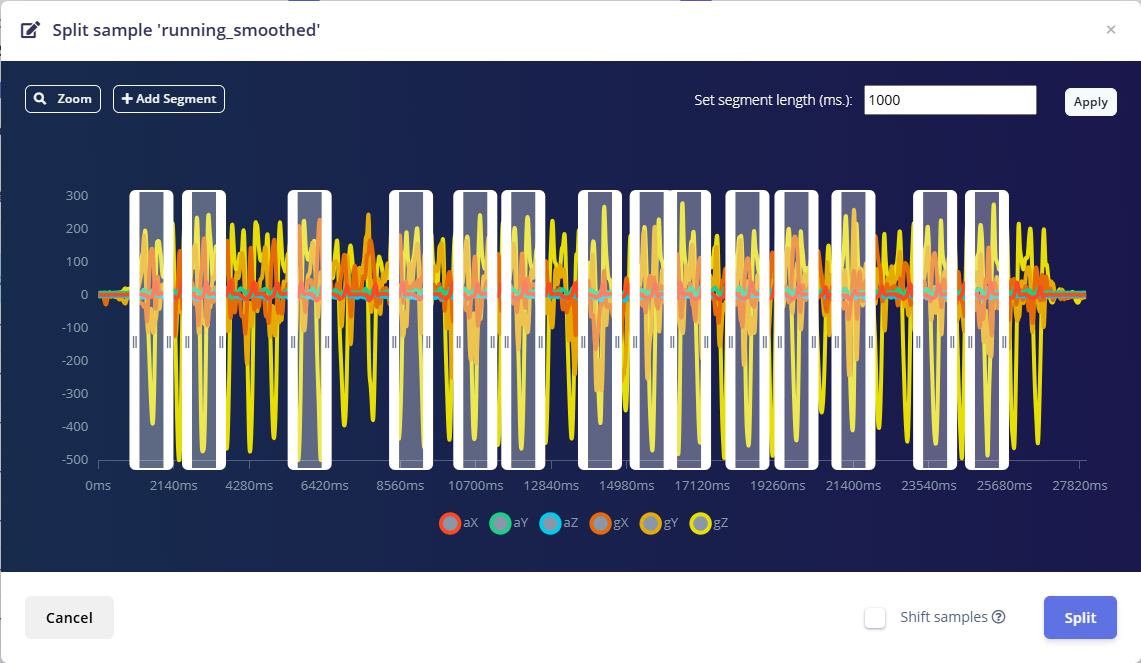
\includegraphics[width=1\linewidth]{images/chapter_3/edgeimpulse_split_sample.png}
        \caption{Edge Impulse Split sample}
        \label{fig:enter-label}
    \end{figure}

    \pagebreak
    After splitting the data into samples, we can finally perform the train/test split to split samples into training dataset and testing dataset.

    \begin{figure}[!htb]
        \centering
        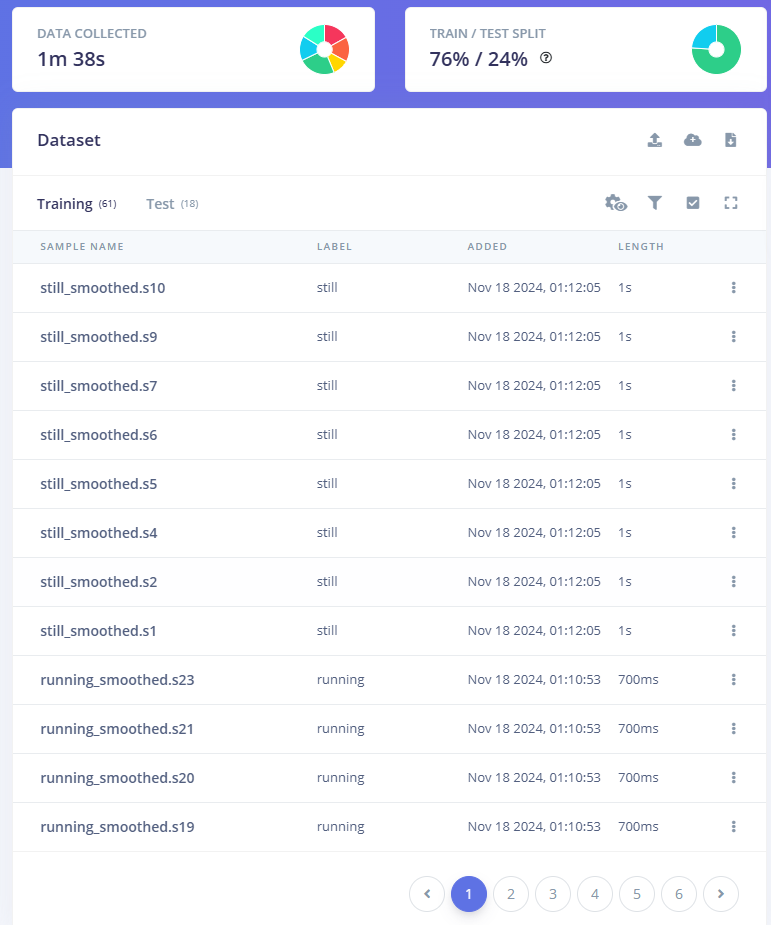
\includegraphics[width=1\linewidth]{images/chapter_3/edgeimpulse_dataset_finish.png}
        \caption{Edge Impulse Final dataset}
        \label{fig:enter-label}
    \end{figure}

\subsection{Impulse creation}
\begin{enumerate}
    \item Create impulse

    First, we need to create an impulse which includes the data specifications block, processing block and learning block.
    
    For the processing block, it is suggested to use the Spectral Analysis because it is great for analyzing repetitive motion, such as data from accelerometers and it extracts the frequency and power characteristics of a signal over time.
    
    For the learning block, using Classification (Keras) is recommended. It learns patterns from data, and can apply these to new data and great for categorizing movement or recognizing audio.
    \begin{figure}[!htb]
        \centering
        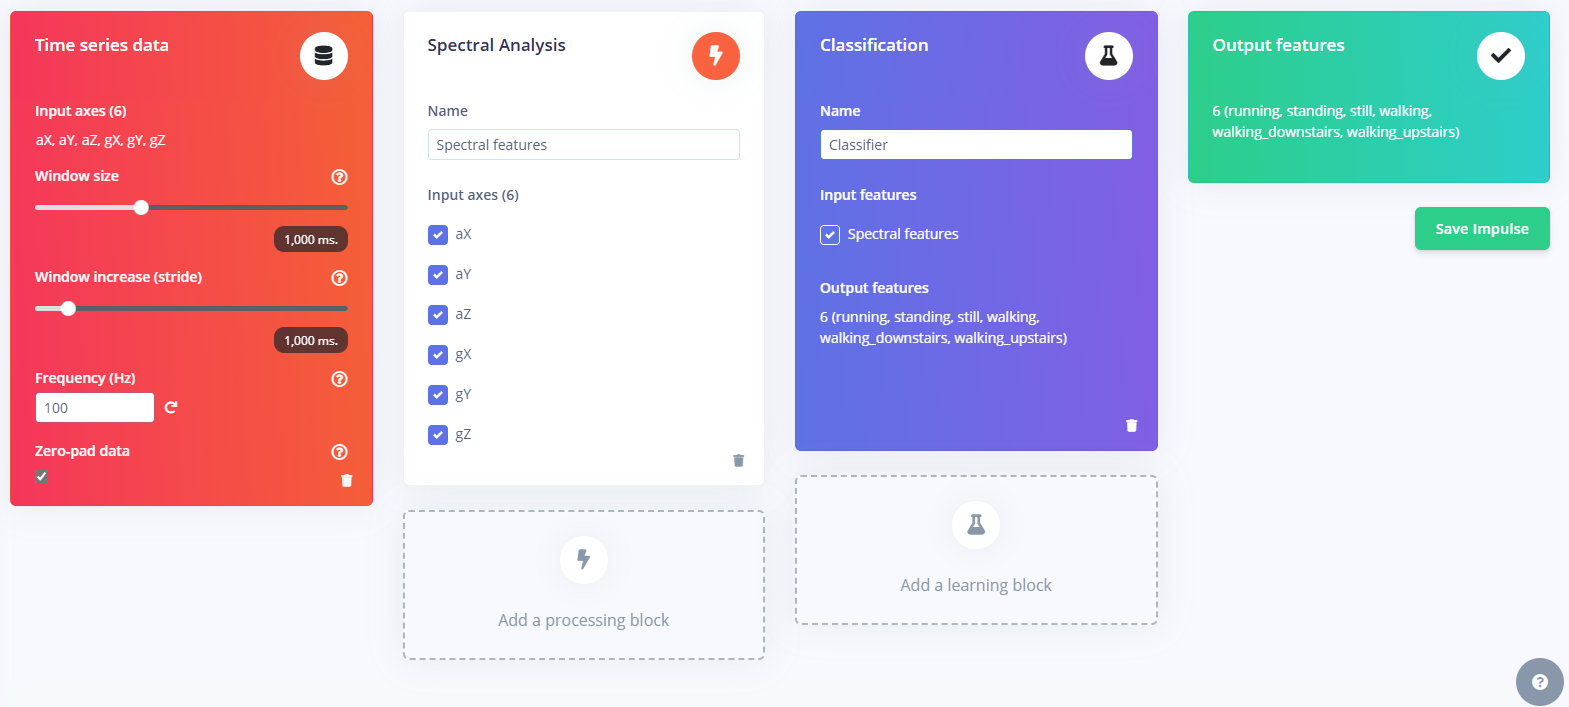
\includegraphics[width=1\linewidth]{images/chapter_3/edgeimpulse_create_impulse.png}
        \caption{Create Impulse}
        \label{fig:enter-label}
    \end{figure}

    \pagebreak
    \item Processing block
    
    Then, by moving to the chosen processing block, we are able to generate features. In this case, the processing block is Spectral features. There are many parameters for us to determine.
    
    \begin{figure}[!htb]
        \centering
        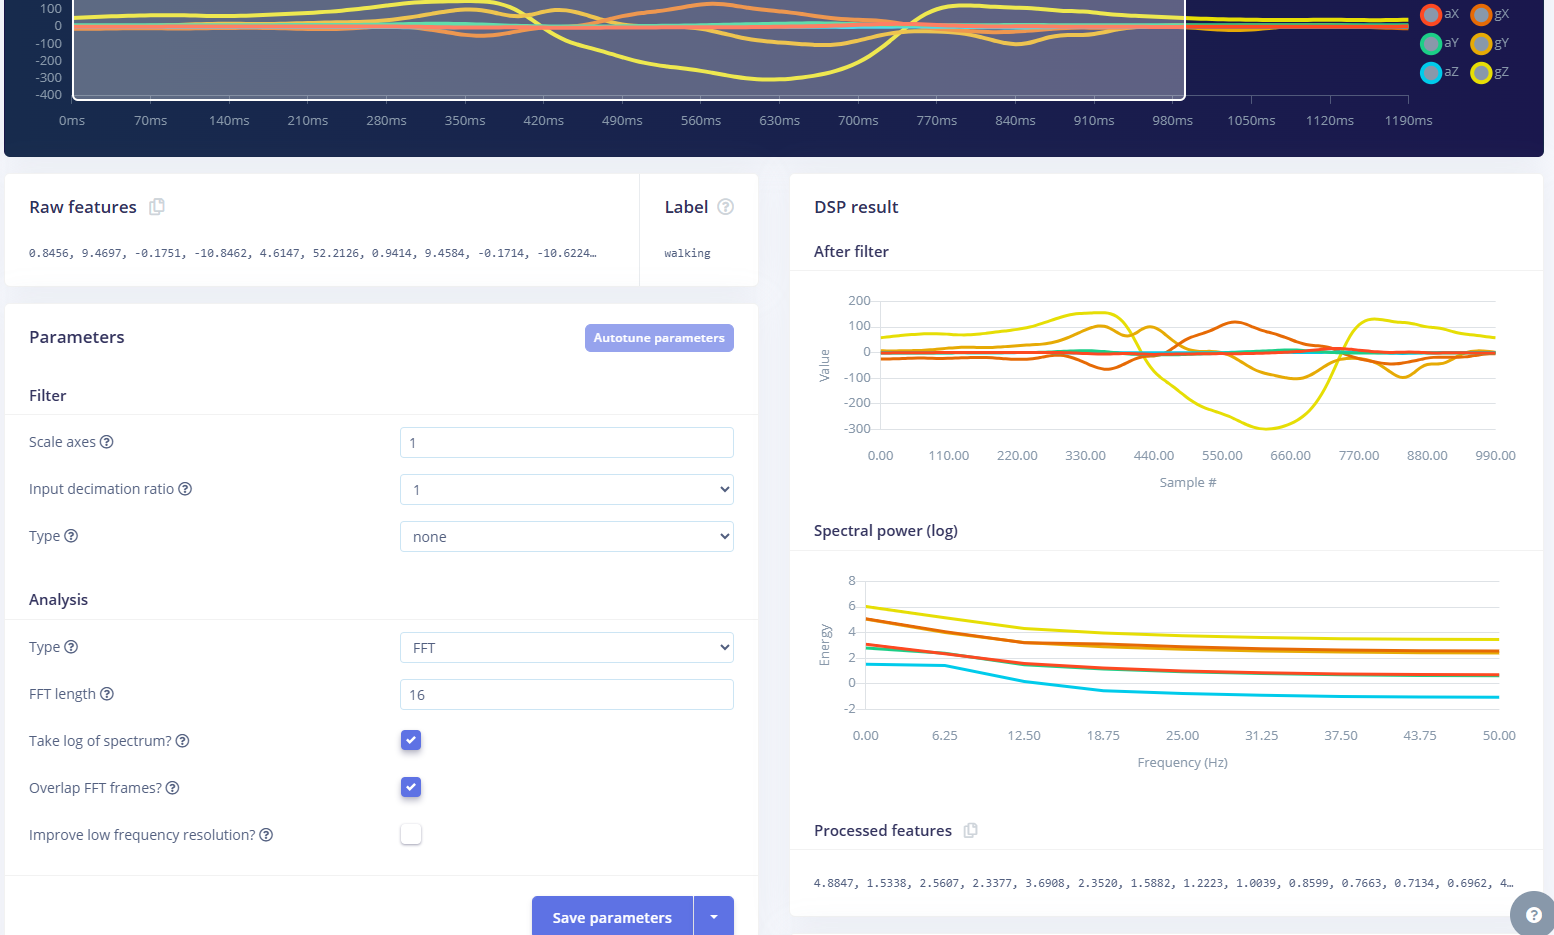
\includegraphics[width=1\linewidth]{images/chapter_3/edgeimpulse_spectral_features_parameters.png}
        \caption{Spectral features parameters}
        \label{fig:enter-label}
    \end{figure}
    
    Once we are satisfied with the parameters, clicking "Save parameters" will direct us to the next panel to generate the features. In this panel, it shows the overall training set information.
    
    \pagebreak
    
    By accepting to generate features, the page will start feature generation job. The output will show the spectrum of the differences between features.

    \begin{figure}[!htb]
        \centering
        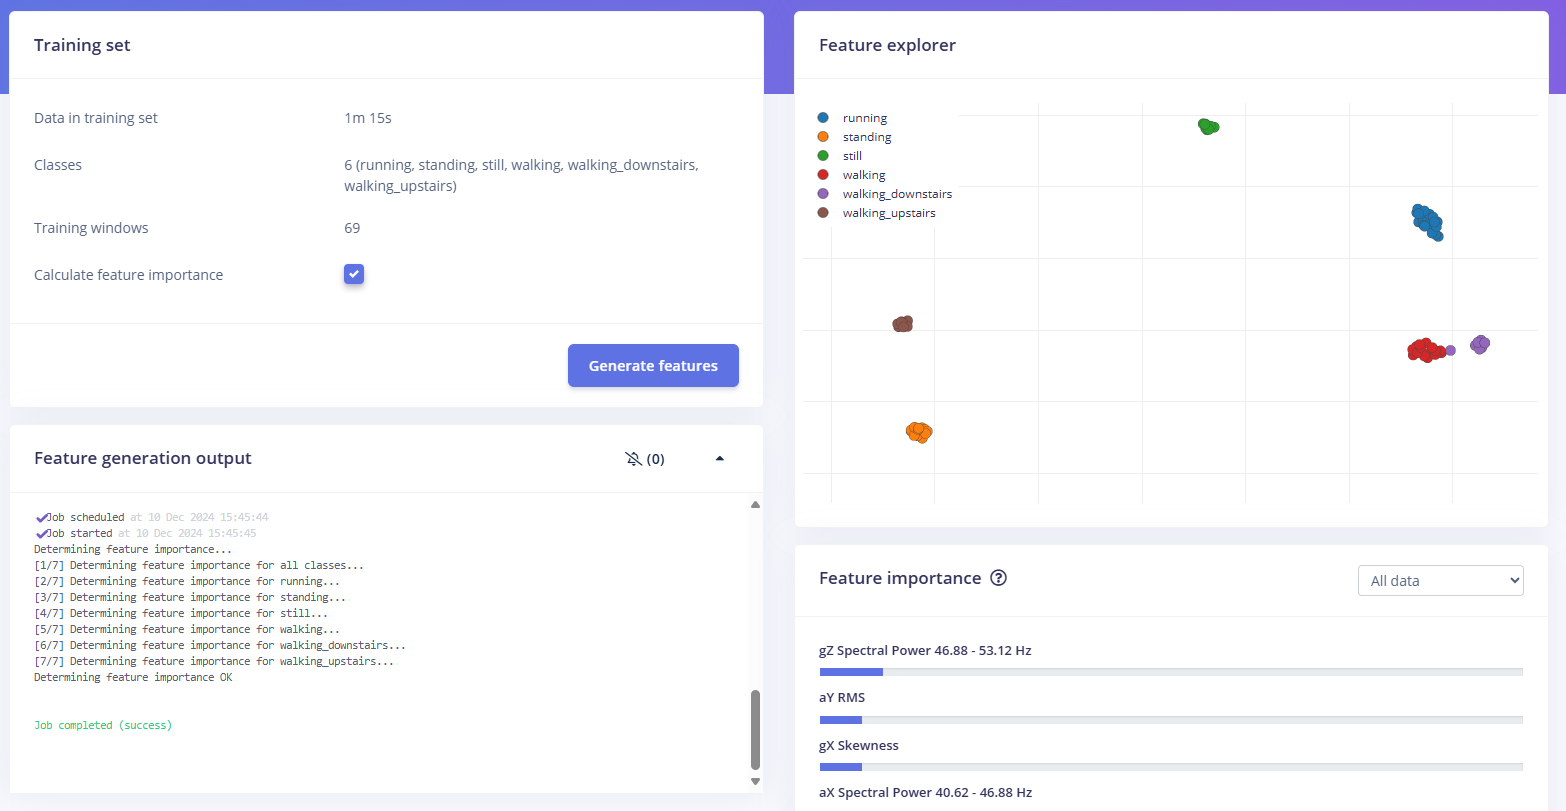
\includegraphics[width=1\linewidth]{images/chapter_3/edgeimpulse_generated_features.png}
        \caption{Generated features}
        \label{fig:edgeimpulse_generated_features}
    \end{figure}
    
    As we can see in \ref{fig:edgeimpulse_generated_features}, most of the features are clearly separated, but the walking feature and walking downstairs feature are near to each other. This will lead to the inaccurate test results between these two.

    \pagebreak

    \item Learning block
    
    Coming to the learning block, we can set the parameters for the neural network settings. 
    
    \begin{figure}[!htb]
        \centering
        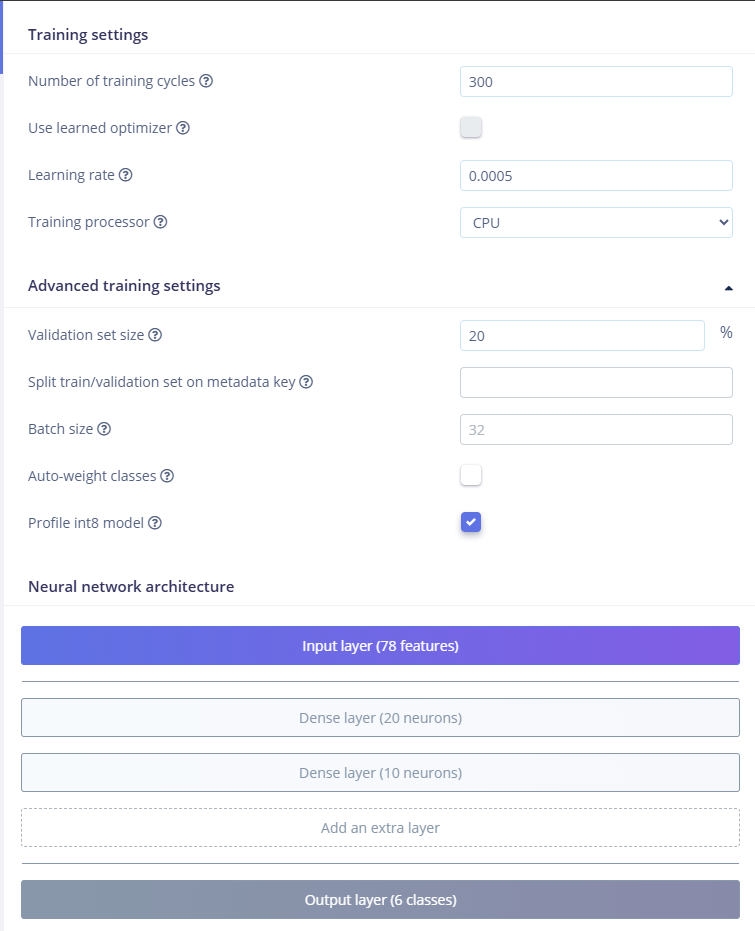
\includegraphics[width=0.8\linewidth]{images/chapter_3/edgeimpulse_neural_network_settings.png}
        \caption{Neural network settings}
        \label{fig:edgeimpulse_neural_network_settings }
    \end{figure}
    
    \pagebreak
    
    After setting the suitable parameters for this part, we can choose "Save and train" for it to start training job. The result of this step will be the confusion matrix, showing that the validation result of the trained model.

    \begin{figure}[!htb]
        \centering
        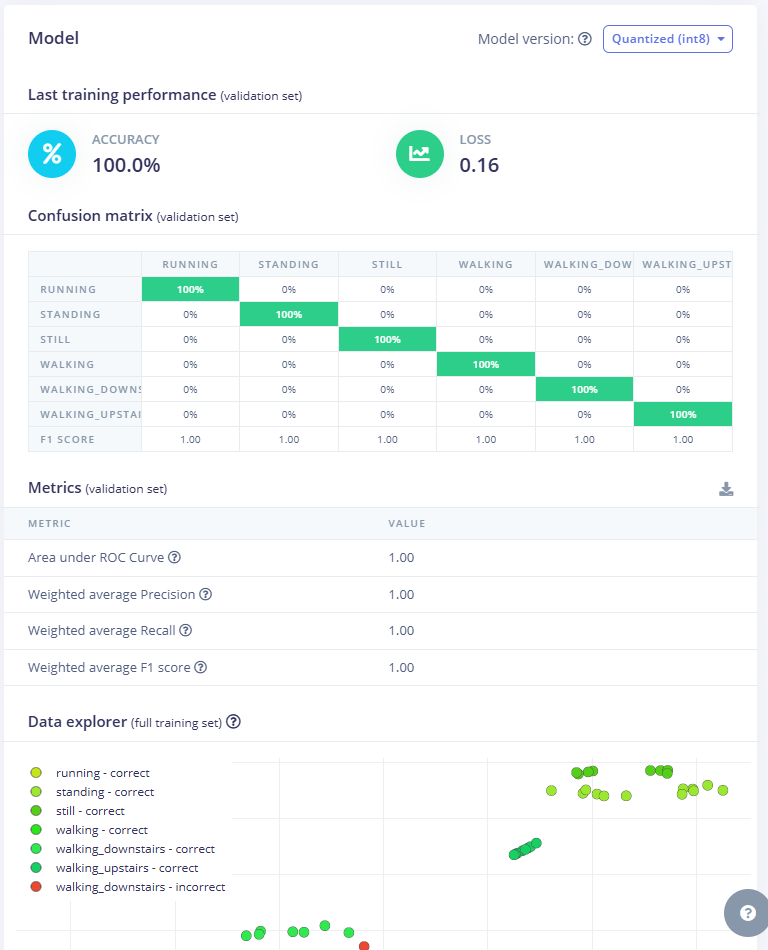
\includegraphics[width=0.75\linewidth]{images/chapter_3/edgeimpulse_trained_model_validation.png}
        \caption{Validation result of trained model}
        \label{fig:edgeimpulse_trained_model_validation}
    \end{figure}
    
    \pagebreak

    \item Model testing
    
    Under the tab for model testing, it is allowed to do the testing on the newly trained model with the testing dataset that we prepared at the beginning.

    \begin{figure}[!htb]
        \centering
        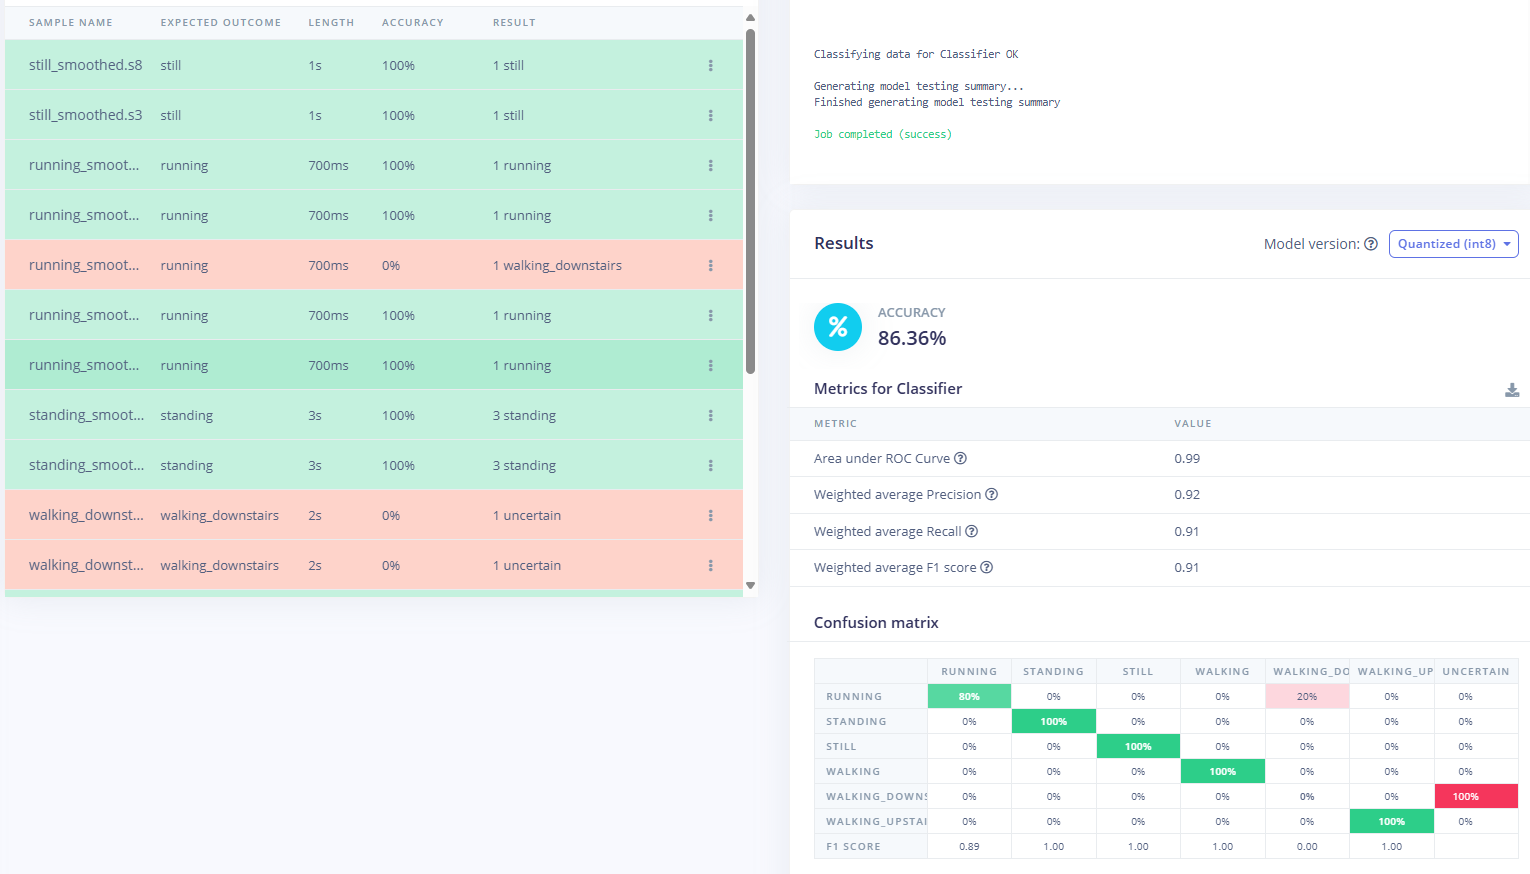
\includegraphics[width=1\linewidth]{images/chapter_3/edgeimpulse_model_testing_output.png}
        \caption{Model testing output}
        \label{fig:edgeimpulse_model_testing_output}
    \end{figure}
    
    As the result, the accuracy is 86.36\%, which is not ideal. The result shows that 100\% of testing results on walking downstairs feature are uncertain.

    \item Deployment
    
    There are various options for deployment target. In this case, we will use the "Arduino library" and the target device is "Nordic nRF52840 DK (Cortex-M4F 64MHz).
    After building, the page will allow us to download the generated model.

    In order to import the generated model to Arduino project, we can use "Add .ZIP library" option in Arduino IDE.
    
    After importing the model, we can include the header file in the Arduino motion prediction project.
\end{enumerate}

\section{Results}
\subsection{Experiment results}
After compiling a simple application to predict motions with the same setup for the ankle-mount device and flashing to the device, it is able to predict some types of motion but not all.

\begin{figure}[htb]
    \centering
    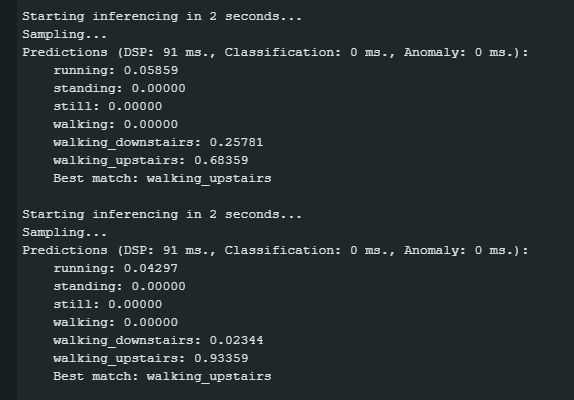
\includegraphics[width=1\linewidth]{images/chapter_3/results_motion_detection.png}
    \caption{Motion detection results}
    \label{fig:results_motion_detection}
\end{figure}

In \ref{fig:results_motion_detection}, the logs are showing the matching percentage for each activity and the best match for the prediction.

The results are telling that the "walking" motion is not detected, and mistaken to "walking{\_}downstairs" or "walking{\_}upstairs". Otherwise, the actual motions "walking{\_}downstairs" and "walking{\_}upstairs" are usually correct, but not always. Finally, the motions as "running", "standing" or "still" are highly accurate.

The inaccurate result is foreseen in the  \ref{fig:edgeimpulse_model_testing_output}. Reasons for this can be from the source of the data, the preprocessing process, the data split methods, or anything that is in the way to create the complete application. Then, we can see the way to improve this is to minimize the possible errors can be caused during the process to produce the final application.

\subsection{Edge Impulse assessments}
Pros:
\begin{itemize}
    \item Ease of Use: User-friendly interface and streamlined workflow for building machine learning models without needing deep expertise in data science.
    \item Optimized for Edge Devices: Designed to optimize models for edge devices with limited resources, ensuring efficient deployment.
    \item Wide Hardware Support: Compatible with a variety of edge devices and sensors, making it versatile for many IoT applications.
    \item Automated Model Optimization: Simplifies model training and optimization for resource-constrained environments, reducing manual effort.
    \item Cloud-Based: Allows for easy collaboration and access to tools from anywhere with an internet connection.
    \item Free Tier Available: Offers a free version with useful features for smaller projects or testing.
    \item Built-In Data Collection Tools: Includes built-in tools for collecting and labeling data directly from sensors, reducing setup time.
    \item Deployment Flexibility: Supports deployment to multiple platforms (e.g., microcontrollers, mobile devices) with minimal setup.
\end{itemize}
Cons:
\begin{itemize}
    \item Limited Customization: Less flexibility for advanced users who need fine-grained control over model architecture or training techniques.
    \item Dependency on Internet: Requires a stable internet connection for training and deployment, which may not be ideal for all environments.
    \item Resource Limitations for Complex Models: Performance may suffer when deploying large or computationally demanding models due to the resource constraints of edge devices.
    \item Challenges with Niche Hardware: Integrating with custom or non-standard hardware may require additional work or custom development.
    \item Paid Features for Scale: Advanced features and scaling capabilities require a paid subscription, which can become expensive for large projects.
    \item Data Privacy Concerns: Cloud-based nature could raise privacy or compliance concerns, particularly for sensitive data.
    \item Learning Curve for Beginners: While user-friendly, beginners without machine learning experience may still face challenges in data collection, labeling, and model creation.
    \item Integration Issues: Integrating Edge Impulse with existing systems or DevOps pipelines can require extra effort or may not always be straightforward.
    \item Limited Model Types: Certain advanced machine learning models (e.g., reinforcement learning) may not be well-supported, limiting its use for highly specialized applications.
\end{itemize}

Conclusion:

Edge Impulse is a powerful tool for simplifying machine learning on edge devices, especially for developers working with IoT or embedded systems. It excels in ease of use, optimization for resource-constrained environments, and hardware support. However, its limitations in customization, dependency on the cloud, and challenges with complex models may make it less suitable for highly specialized or large-scale projects.